% ------------------------------------------------------------------------------
% FORMATVORLAGE DOKU/ BEDIENUNGSANLEITUNG
% ------------------------------------------------------------------------------

% DOKUMENTENKOPF ---------------------------------------------------------------
%   Diese Vorlage basiert auf "scrreprt" aus dem koma-script.
% ------------------------------------------------------------------------------
\documentclass[
    11pt,    % Schriftgr��e
    DIV10,
    ngerman, % f�r Umlaute, Silbentrennung etc.
    a4paper, % Papierformat
    oneside, % einseitiges Dokument
    titlepage, % es wird eine Titelseite verwendet
    parskip=half, % Abstand zwischen Abs�tzen (halbe Zeile)
    headings=normal, % Gr��e der �berschriften verkleinern
    listof=totoc, % Verzeichnisse im Inhaltsverzeichnis auff�hren
    bibliography=totoc, % Literaturverzeichnis im Inhaltsverzeichnis auff�hren
    index=totoc, % Index im Inhaltsverzeichnis auff�hren
    captions=tableheading, % Beschriftung von Tabellen unterhalb ausgeben
    final % Status des Dokuments (final/draft)
]{scrreprt}

% globale Definitionen -----------------------------------------------------------
%   Informationen �ber das Dokument, wie z.B. Titel, Autor, Datum 
%   werden in der Datei globale_Definitionen.tex definiert und k�nnen danach global
%   verwendet werden.
% ------------------------------------------------------------------------------
% Meta-Informationen -----------------------------------------------------------
%   Definition von globalen Parametern, die im gesamten Dokument verwendet
%   werden k�nnen (z.B auf dem Deckblatt etc.).
%
%   ACHTUNG: Wenn die Texte Umlaute oder ein Esszet enthalten, muss der folgende
%            Befehl bereits an dieser Stelle aktiviert werden:
%            \usepackage[latin1]{inputenc}
% ------------------------------------------------------------------------------
\newcommand{\titel}{Umprogrammierung von EPROM-Modulen f�r den {\FLTester}}
\newcommand{\untertitel}{}%{TODO: und hier kommt der Untertitel}
\newcommand{\Bezeichnung}{Module f�r {\FLTester} programmieren}
\newcommand{\BezeichnungLang}{EPROM-Module f�r {\MarelliTester} �ndern}
%\newcommand{\Version}{V0.1}
\newcommand{\Dokumentart}{A N L E I T U N G}
\newcommand{\autor}{schlizb�da}
\newcommand{\jahr}{2016}

% verwendete Hardware
\newcommand{\FLTester}{F/L-Tester}
\newcommand{\MarelliTester}{Fiat Lancia Tester (Magneti Marelli)} % TODO: Internetbilder "FIAT" "LANCIA" "Tester" "MagnetiMarelli" 
\newcommand{\Batronix}{Batronix BARLINO II} % Programmierger�t
% verwendete Software
\newcommand{\ProgExpress}{Prog-Express} % Batronix Programmiersoftware

%%Steuerelemente von Software:
%\newcommand{\prompt}[1]{\Code{\textit{#1}}}
%\newcommand{\filenam}[1]{\Code{#1}}
%
%\newcommand{\button}[1]{\Code{[{#1}]}}
%\newcommand{\menuitem}[1]{\textbf{\textit{"{#1}"}}}
%\newcommand{\checkbox}[1]{\textbf{\textit{"{#1}"}}}

%Smileys:
\newcommand{\smiley}[1]{\includegraphics[width=0.3cm]{Bilder/smileys/{#1}}}


% ben�tigte Packages -----------------------------------------------------------
%   LaTeX-Packages, die ben�tigt werden, sind in die Datei Packages.tex
%   "ausgelagert", um diese Vorlage m�glichst �bersichtlich zu halten.
% ------------------------------------------------------------------------------
% Anpassung des Seitenlayouts --------------------------------------------------
%   siehe Seitenstil.tex
% ------------------------------------------------------------------------------
\usepackage[
    automark, % Kapitelangaben in Kopfzeile automatisch erstellen
    headsepline, % Trennlinie unter Kopfzeile
    ilines % Trennlinie linksb�ndig ausrichten
]{scrpage2}

% Anpassung an Landessprache ---------------------------------------------------
\usepackage[ngerman]{babel}

% Umlaute ----------------------------------------------------------------------
%   Umlaute/Sonderzeichen wie ���� direkt im Quelltext verwenden (CodePage).
%   Erlaubt automatische Trennung von Worten mit Umlauten.
% ------------------------------------------------------------------------------
\usepackage[latin1]{inputenc}
%\usepackage[utf8]{inputenc}
\usepackage[T1]{fontenc}
\usepackage{textcomp} % Euro-Zeichen,Copyright etc.

% Schrift ----------------------------------------------------------------------
\usepackage{lmodern} % bessere Fonts
\usepackage{relsize} % Schriftgr��e relativ festlegen

% Grafiken ---------------------------------------------------------------------
% Einbinden von JPG-Grafiken erm�glichen
\usepackage[dvips,final]{graphicx}
% hier liegen die Bilder des Dokuments
\graphicspath{{Bilder/}}

% Befehle aus AMSTeX f�r mathematische Symbole z.B. \boldsymbol \mathbb --------
\usepackage{amsmath,amsfonts}

% f�r Index-Ausgabe mit \printindex --------------------------------------------
\usepackage{makeidx}

% Einfache Definition der Zeilenabst�nde und Seitenr�nder etc. -----------------
\usepackage{setspace}
\usepackage{geometry}

% ------------------------------------------------------------------------------
% --- Abk�rzungsverzeichnis ----------------------------------------------------
% ------------------------------------------------------------------------------
%   Symbolverzeichnisse bequem erstellen. Beruht auf MakeIndex:
%     makeindex.exe %Name%.nlo -s nomencl.ist -o %Name%.nls
%   erzeugt dann das Verzeichnis. Dieser Befehl kann z.B. im TeXnicCenter
%   als Postprozessor eingetragen werden, damit er nicht st�ndig manuell
%   ausgef�hrt werden muss.
%   Die Definitionen sind ausgegliedert in die Datei "Glossar.tex".
% ------------------------------------------------------------------------------
\usepackage[intoc]{nomencl}
\let\abbrev\nomenclature
\renewcommand{\nomname}{Abk�rzungsverzeichnis}
\setlength{\nomlabelwidth}{.25\hsize}
\renewcommand{\nomlabel}[1]{#1 \dotfill}
\setlength{\nomitemsep}{-\parsep}

\usepackage{acronym}


% zum Umflie�en von Bildern ----------------------------------------------------
\usepackage{floatflt}

% ------------------------------------------------------------------------------
% --- Listings zum einbinden von CODE ------------------------------------------
% ------------------------------------------------------------------------------
\usepackage{listings}
\usepackage[table]{xcolor} 
% Farben f�r listenings definieren! alternativ: {RGB}{0-255,0-255.0-255}
\definecolor{hellgelb}{rgb}{1,1,0.9}			     
\definecolor{colKeys}{rgb}{0,0,1}
\definecolor{colIdentifier}{rgb}{0,0,0}
\definecolor{colComments}{rgb}{0,0.5,0.1} 
\definecolor{colString}{rgb}{1,0,0}
\lstset{
    float=hbp,
    basicstyle=\ttfamily\color{black}\small\smaller, % the size of the fontsthat are used for the code 
    identifierstyle=\color{colIdentifier},
    keywordstyle=\color{colKeys},
    stringstyle=\color{colString},
    commentstyle=\color{colComments},
    columns=flexible,
    tabsize=3,
    %frame=single,                     % add frame arround the code
    extendedchars=true,
    showspaces=false,
    showstringspaces=false,
    numbers=left,                      % where to put the line numbers
    numberstyle=\tiny,                % fontsize for line
    stepnumber= 1,                     % stepnumber between line-numbers
    breaklines=true,                   % sets automatic line breaking
    captionpos=b,                      % sets caption position to bottom
    backgroundcolor=\color{hellgelb},
    breakautoindent=true,
    }

% URL verlinken, lange URLs umbrechen etc. -------------------------------------
\usepackage{url}

% wichtig f�r korrekte Zitierweise ---------------------------------------------
\usepackage[numbers]{natbib}  % [square] to [numbers] jetzt gehen versch. stile

% ------------------------------------------------------------------------------
% --- PDF Optionen -------------------------------------------------------------
% ------------------------------------------------------------------------------
\definecolor{darkblue}{rgb}{0,0,0.5} % def. Farbe f�r PDF Verlinkungen
\usepackage[
    bookmarks,
    bookmarksopen=true,
    colorlinks=true,
% diese Farbdefinitionen zeichnen Links im PDF farblich aus
    linkcolor=darkblue,% einfache interne Verkn�pfungen
    anchorcolor=black,% Ankertext
    citecolor=blue,   % Verweise auf Literaturverzeichniseintr�ge im Text
    filecolor=magenta,% Verkn�pfungen, die lokale Dateien �ffnen
    menucolor=red,    % Acrobat-Men�punkte
    urlcolor=cyan, 
% diese Farbdefinitionen sollten f�r den Druck verwendet werden (alles schwarz)
    %linkcolor=black,  % einfache interne Verkn�pfungen
    %anchorcolor=black,% Ankertext
    %citecolor=black,  % Verweise auf Literaturverzeichniseintr�ge im Text
    %filecolor=black,  % Verkn�pfungen, die lokale Dateien �ffnen
    %menucolor=black,  % Acrobat-Men�punkte
    %urlcolor=black, 
    backref,
    plainpages=false, % zur korrekten Erstellung der Bookmarks
    pdfpagelabels, % zur korrekten Erstellung der Bookmarks
    hypertexnames=false, % zur korrekten Erstellung der Bookmarks
    linktocpage % Seitenzahlen anstatt Text im Inhaltsverzeichnis verlinken
]{hyperref}
% Befehle, die Umlaute ausgeben, f�hren zu Fehlern, wenn sie hyperref als Optionen �bergeben werden
\hypersetup{
    pdftitle={\titel \untertitel},
    pdfauthor={\autor},
    pdfcreator={\autor},
    pdfsubject={\titel \untertitel},
    pdfkeywords={\titel \untertitel},
}

% fortlaufendes Durchnummerieren der Fu�noten ----------------------------------
\usepackage{chngcntr}

% f�r lange Tabellen -----------------------------------------------------------
\usepackage{longtable}
\usepackage{array}
\usepackage{ragged2e}
\usepackage{lscape}

% Spaltendefinition rechtsb�ndig mit definierter Breite ------------------------
\newcolumntype{w}[1]{>{\raggedleft\hspace{0pt}}p{#1}}

% Formatierung von Listen �ndern -----------------------------------------------
\usepackage{paralist}

% bei der Definition eigener Befehle ben�tigt
\usepackage{ifthen}

% definiert u.a. die Befehle \todo und \listoftodos
\usepackage{todonotes}

% sorgt daf�r, dass Leerzeichen hinter parameterlosen Makros nicht als Makroendezeichen interpretiert werden
\usepackage{xspace}

% zur Formatierung der Abbildungsunterschriften (Captions)
\usepackage{caption}
\captionsetup{labelfont=bf,textfont=it} % Abbildung fett, Text kursiv

% zum Einbinden von Messageboxen 
\usepackage[tikz]{bclogo}

% zum Formatieren von Tabellen
\usepackage{booktabs}
\renewcommand{\arraystretch}{1}% Zeilenabstand in einer Tabelle auf 2

% zum Einbinden von PDF Dateien
\usepackage{pdfpages}


% Erstellung eines Index und Abk�rzungsverzeichnisses aktivieren ---------------
\makeindex
\makenomenclature

% Kopf- und Fu�zeilen, Seitenr�nder etc. ---------------------------------------


% Zeilenabstand 1,5 Zeilen -----------------------------------------------------
\onehalfspacing

% ------------------------------------------------------------------------------
% ----------- Seitenr�nder -----------------------------------------------------
% ------------------------------------------------------------------------------

\setlength{\topskip}{\ht\strutbox} % behebt Warnung von geometry
\geometry{paper=a4paper,left=30mm,right=25mm,top=20mm,bottom=40mm}
% zus�tzlich bindingoffset angebbar(linker Rand)

% ------------------------------------------------------------------------------
% ----------- Kopf- und Fu�zeilen ----------------------------------------------
% ------------------------------------------------------------------------------

\pagestyle{scrheadings}
% Kopf- und Fu�zeile auch auf Kapitelanfangsseiten
\renewcommand*{\chapterpagestyle}{scrheadings} 
% Schriftform der Kopfzeile
\renewcommand{\headfont}{\normalfont}

%%% KOPFZEILE %%%
\ihead{\hspace*{16pt} \large{\textsc{\titel}} \\[1ex] \textit{\hspace*{16pt} \headmark}}
\chead{}
%\ohead{\includegraphics[scale=0.06]{\logo}}
\setlength{\headheight}{21mm}           % H�he der Kopfzeile
% Kopfzeile �ber den Text hinaus verbreitern
\setheadwidth[-20pt]{textwithmarginpar} % neg. schiebt nach links, 0 is mittig
\setheadsepline[text]{0.4pt}[\hspace{20pt}]    % Trennlinie unter Kopfzeile [text,head,]

%%% FU�ZEILE %%%
\ifoot{}  %\ifoot{\copyright\ \autor} Autor optional hinzuf�gen
\cfoot{- \pagemark ~-}
\ofoot{}

% ------------------------------------------------------------------------------
% ----------- sonstige typographische Einstellungen ----------------------------
% ------------------------------------------------------------------------------

\frenchspacing % erzeugt ein wenig mehr Platz hinter einem Punkt

% Schusterjungen und Hurenkinder vermeiden
\clubpenalty = 10000
\widowpenalty = 10000 
\displaywidowpenalty = 10000

% Quellcode-Ausgabe formatieren
\lstset{numbers=left, numberstyle=\tiny, numbersep=5pt, breaklines=true}
\lstset{emph={square}, emphstyle=\color{red}, emph={[2]root,base}, emphstyle={[2]\color{blue}}}

% Fu�noten fortlaufend durchnummerieren
\counterwithout{footnote}{chapter}

%\parindent 0pt % kein Einzug nach NewLine

% eigene LaTeX-Befehle
% Eigene Befehle und typographische Auszeichnungen f�r diese Arbeit
% ------------------------------------------------------------------------------

% einfaches Wechseln der Schrift, z.B.: \changefont{cmss}{sbc}{n}
\newcommand{\changefont}[3]{\fontfamily{#1} \fontseries{#2} \fontshape{#3} \selectfont}

% ------------------------------------------------------------------------------
% Abk�rzungen mit korrektem Leerraum 
%-------------------------------------------------------------------------------
\newcommand{\ua}{\mbox{u.\,a.\ }}
\newcommand{\zB}{\mbox{z.\,B.\ }}
\newcommand{\dahe}{\mbox{d.\,h.\ }}
\newcommand{\Vgl}{Vgl.\ }
\newcommand{\bzw}{bzw.\ }
\newcommand{\evtl}{evtl.\ }

\newcommand{\abbildung}[1]{Abbildung~\ref{fig:#1}}

\newcommand{\bs}{$\backslash$}

% erzeugt ein Listenelement mit fetter �berschrift 
\newcommand{\itemd}[2]{\item{\textbf{#1}}\\{#2}}

% -----------------------------------------------------------------------------
% einige Befehle zum Zitieren
% -----------------------------------------------------------------------------
\newcommand{\Zitat}[2][\empty]{\ifthenelse{\equal{#1}{\empty}}{\citep{#2}}{\citep[#1]{#2}}}

% zum Ausgeben von Autoren
\newcommand{\AutorName}[1]{\textsc{#1}}
\newcommand{\Autor}[1]{\AutorName{\citeauthor{#1}}}

% -----------------------------------------------------------------------------
% verschiedene Befehle um W�rter semantisch auszuzeichnen
% -----------------------------------------------------------------------------
\newcommand{\NeuerBegriff}[1]{\textbf{#1}}
\newcommand{\Fachbegriff}[1]{\textit{#1}}

\newcommand{\Eingabe}[1]{\texttt{#1}}
\newcommand{\Code}[1]{\texttt{#1}}
\newcommand{\Datei}[1]{\texttt{#1}}

\newcommand{\Datentyp}[1]{\textsf{#1}}
\newcommand{\XMLElement}[1]{\textsf{#1}}
\newcommand{\Webservice}[1]{\textsf{#1}}


% DAS EIGENTLICHE DOKUMENT -----------------------------------------------------
%   Der eigentliche Inhalt des Dokuments beginnt hier. Die einzelnen Seiten
%   und Kapitel werden in eigene Dateien ausgelagert und hier nur inkludiert.
% ------------------------------------------------------------------------------
% ------------------------------------------------------------------------------
\begin{document}

% auch subsubsection nummerieren
\setcounter{secnumdepth}{3}
\setcounter{tocdepth}{3}

% Seitennummerierung -----------------------------------------------------------
%   Vor dem Hauptteil werden die Seiten in gro�en r�mischen Ziffern 
%   nummeriert.
% ------------------------------------------------------------------------------
\pagenumbering{Roman}

% Deckblatt und Abstract ohne Seitenzahl
\cfoot{}
% -- Deckblatt.tex -----------------------------------------------------------
%
%   Gestaltung des Deckblattes der Bedienungsanleitung:  
%   - Einbinden und formatieren der Logos
%   - Bezeichnungen befinden sich in 'Meta.tex'   
% ------------------------------------------------------------------------------

\thispagestyle{empty} % von plain nach empty
\begin{titlepage}
\vspace*{-3cm}% vertikale negative Verschiebung
%%------------------------------------------------------------------------------
%%   Firmenlogo einf�gen
%%------------------------------------------------------------------------------
\begin{figure}[h]
\centering

\includegraphics[width=0.25\textwidth]{schlizbaeda.png}
\end{figure}

\begin{center}
\LARGE{\textbf{\Dokumentart}}\\[1.5ex] 
\Large{\BezeichnungLang}\\[4ex]
%%------------------------------------------------------------------------------
%%   Titel der Bedienungsanleitung
%%------------------------------------------------------------------------------
\noindent\rule[1ex]{\textwidth}{3pt} % vertikaler Strich
%\huge{\textbf{\titel}}\\[1.5ex]      % TITEL DER ARBEIT
\textbf{\titel}\\[1.5ex]              % TITEL DER ARBEIT (lange �berschrift)
\noindent\rule[1ex]{\textwidth}{3pt} 
%\LARGE{\textbf{\untertitel}}\\[6ex]
%\LARGE{\textbf{\art}}\\[1.5ex]
%\Large{im Fachgebiet \fachgebiet}
\\[2ex]

\normalsize
%%------------------------------------------------------------------------------
%%   Bild
%%------------------------------------------------------------------------------
\begin{figure}[h]
\centering
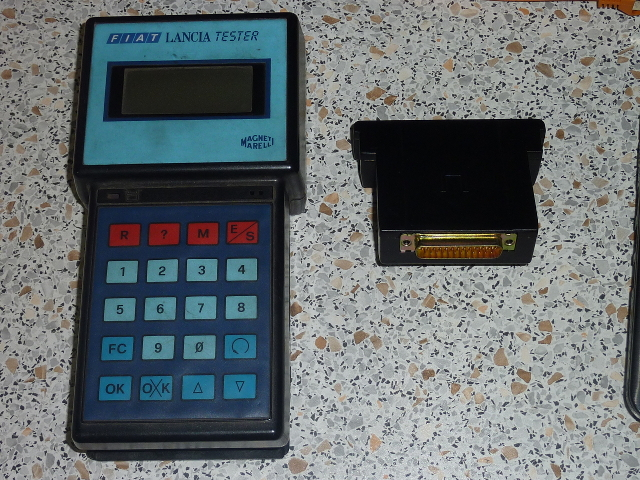
\includegraphics[width=12cm]{Titelbild.JPG}
\end{figure}

%%------------------------------------------------------------------------------
%%   CE und Firmenadresse
%%------------------------------------------------------------------------------
\begin{tabular}{p{3cm} p{8cm} p{3cm}}\\ % die beiden 0.5cm breiten "TabellensSpalten" sind eigentlich latex-unw�rdiges Gepfriemel! Ich kann's aber nicht besser!
\hline
\parbox[c]{75px}{\includegraphics{MagnetiMarelli.png}} & \textbf{Module f�r {\FLTester} programmieren} Datum: 23.10.2016 & \parbox[c]{75px}{\includegraphics{FiatLancia75x75.png}}\\
\hline
\end{tabular}

\end{center}


Diese Anleitung wurde mit dem Textsatzsystem \LaTeX\ erstellt.
%% Das trifft hier nicht zu:
%\textbf{}\\
%Das Bild auf dem Fernsehger�t stammt aus dem Video zu folgendem Musikst�ck:\\
%\texttt{\textbf{Riegler Hias feat. d' Hundskrippln} \textit{Gloana Bauer}} bei 0:15\\
%\url{http://www.hundskrippln.de/#filme}
\end{titlepage}




\include{Layout/Abstract}
\cfoot{- \pagemark ~-}

\tableofcontents          % Inhaltsverzeichnis
\listoffigures            % Abbildungsverzeichnis
\listoftables             % Tabellenverzeichnis
\renewcommand{\lstlistlistingname}{Verzeichnis der Listings}
%\lstlistoflistings        % Listings-Verzeichnis

% Abk�rzungsverzeichnis --------------------------------------------------------
%% Abk�rzungsverzeichnis:
%% --------------------------------------------------------------------
%\nomenclature{API}{Application Programming Interface}
%\nomenclature{ARIS}{Architektur integrierter Informationssysteme}
%\nomenclature{BPR}{Business Process Reengineering}
%\nomenclature{eEPK}{erweiterte Ereignisgesteuerte Prozesskette}
%\nomenclature{EPK}{Ereignisgesteuerte Prozesskette}
%\nomenclature{JMS}{Java Message Service}
%\nomenclature{SDK}{Software Development Kit}
%\nomenclature{URI}{Uniform Resource Identifier}
%\nomenclature{URL}{Uniform Resource Locator}
%\nomenclature{URN}{Uniform Resource Name}
%\nomenclature{W3C}{World Wide Web Consortium}
%\nomenclature{XML}{Extensible Markup Language}
%\nomenclature{XPath}{XML Path Language}
%\nomenclature{XSL}{Extensible Stylesheet Language}
%\nomenclature{XSLT}{XSL Transformations}

%\begin{itemize}
%\item	gLOSSAR1
%\item	Glossar2
%\end{itemize}

% f�r korrekte �berschrift in der Kopfzeile
\clearpage\markboth{\nomname}{\nomname} 
\printnomenclature
\label{sec:Glossar}


% arabische Seitenzahlen im Hauptteil ------------------------------------------
\clearpage
\pagenumbering{arabic}


% ##############################################################################
% ----------   Die Inhaltskapitel werden inkludiert    -------------------------
% ##############################################################################
\chapter{Einf�hrung}
\label{cha:Einfuehrung}

\section{ACHTUNG}
{\LARGE Stand 16.05.2017

Leider sehe ich mich derzeit nicht in der Lage, meine Erkenntnisse rechtlich 
gefahrlos zu ver�ffentlichen! Ich werde versuchen, �ber offizielle Stellen des
FIAT-Konzerns die Erlaubnis zu erlangen, dies doch ver�ffentlichen zu d�rfen.
Bis zur Kl�rung dieses Sachverhalts sehe ich mich gezwungen,
meine Arbeit vorerst teilweise zur�ckzuziehen.

Vielen Dank f�r Ihr Verst�ndnis.


schlizbaeda@gmx.de}
\newpage

\section{Kurzbeschreibung und technische Daten des {\FLTester}s}
Der {\FLTester} ist ein elektronisches Diagnoseger�t f�r Kraftfahrzeuge
der FIAT-Gruppe: Es ist ein tragbarer Computer (basierend auf dem
8bit-Mikroprozessor Hitachi HD6303RP), der den Datenaustausch mit den in
den Fahrzeugen eingebauten elektronischen Steuerger�ten erm�glicht.\\
Die Software (Pr�fprogramm) wird dem {\FLTester} �ber ein EPROM-Modul
zugef�hrt, das abh�ngig vom zu pr�fenden Steuerger�tetyp ausgew�hlt
und gesteckt werden muss.

Auszug aus der Original-Betriebsanleitung:\\
\textit{Das Diagnoseger�t kann die betreffenden Daten des zu
analysierenden Systems auswerten und speichern, und so dem Operator �ber
ein Display geeignete Instruktionen zur Analyse eventueller
Fehlfunktionen und zur Auffindung der besch�digten Komponenten geben.\\
Der Tester erkennt automatisch den Steuerger�tetyp, an den er
angeschlossen ist. Die Verbindung mit dem Bord-Steuerger�t erfolgt durch
einen spezifischen Standardstecker (siehe Abb. 1).\\
Das Testger�t kann au�erdem die Informationen an verschiedene Terminals
weiterleiten (Drucker, Monitor, zentrale Computer u.\,s.\,w.).}

\subsection*{Technische Daten}
\begin{tabular}{ll}
Stromversorgung:          & 7 -- 30V dc\\
Arbeitstemperatur:        & 0 -- 70�C\\
Format der Diagnosecodes: & NRZ, PCM, Zweiphasen\\
Eingangsfrequenz:         & 1Hz -- 10kHz\\
Zus�tzlicher Ausgang:     & RS232 (50 -- 19200bps)\\
Display:                  & alphanumerisches LCD, 4 Zeilen � 16 Zeichen\\
CPU:                      & Hitachi HD6303RP (8bit, 1MHz)\\
Speicherkapazit�t RAM:    & 2K/8KByte mit permanenter Datenspeicherung\\
Speicherkapazit�t ROM:    & max. 136KByte (abh�ngig vom EPROM-Modul)\\
\end{tabular}
\\

Der Aufbau entspricht dem technischen Stand der Heimcomputer aus den
fr�hen 1980er-Jahren wie \zB dem Commodore 64. Die Entwicklung des
{\FLTester}s d�rfte etwa um 1990 erfolgt sein. Auf einigen vorliegenden
Modulen lassen die Beschriftungen auf ein Herstelldatum von 1995 \bzw
1996 schlie�en. 


\section{Aufbau der EPROM-Module}
Die EPROM-Module bestehen aus einer Leiterplatte, die mit drei EPROM-ICs
vom Typ 27C512 (512kBit, 64KByte) ist. Bei IC1 sind die drei oberen
Adressleitungen (A13, A14 und A15) fest mit GND verbunden, so dass
dieser EPROM nur mit max. 8KByte Daten bef�llt werden kann. Um dem
{\FLTester}, der eigentlich nur 64KByte adressieren kann, einen gr��eren
Programmspeicher zur Verf�gung zu stellen, befindet sich auf den Modulen
eine zus�tzliche ChipEnable-Logik, die �ber einen 74HC00 (NAND-Gatter)
umgesetzt ist. Damit kann der {\FLTester} �ber dieses "`Banking"' bis zu
136KByte ROM-Speicher adressieren.

Von den Leiterplatten der EPROM-Module gibt es mindestens drei
Layoutvarianten:\\
\begin{tabular}{ll}
\textbf{79 54 33 50}: & Best�ckung mit kleineren EPROMs bis M27C256\\
                      & wurde f�r die ersten Module mit den niedrigen Nummern verwendet\\
                      & \zB M1C, M2B, M3B, \textbf{M6B}, M7A \ua(?)\\
\textbf{79 63 15 40}: & Best�ckung mit 64KByte-EPROMs (M27C512)\\
                      & Diese Variante wurde schaltungstechnisch (noch) nicht untersucht\\
                      & gefunden auf den Modulen M12A und M15A\\
                      & $\rightarrow$ Die Daten konnten problemlos ausgelesen werden.\\
\textbf{79 63 82 40}: & h�ufigstes Modul, Best�ckung mit 64KByte-EPROMs (M27C512)\\
                      & vermutlich der aktuelle Designstand\\
                      & Alle sp�teren Module (\zB \textbf{M23A}) verwenden dieses Layout\\
\end{tabular}
\\

Die Stromlaufpl�ne der EPROM-Module befinden sich im Anhang.


\section{Liste der EPROM-Module}
\begin{table}[!h]
%\centering
\renewcommand{\arraystretch}{1.2}
\begin{tabular}{|l|l|l|}
\hline%\toprule[2pt]
\textbf{Modul} & \textbf{Bemerkung}              & \textbf{Fahrzeugtyp(en) (unvollst�ndig)}\\ 
\hline%\midrule[2pt]
M1C            & IAW, SPI-GM                     & Delta GT i.e. 8V Kat\\
\hline
M2B            & Digiplex 2, Microplex           & \\
\hline
M3B            & Bosch Monojetronic, L3.1 / L3.2 & \\
\hline
M4B            & S.C.S. / S.I. Fahrwerk          & \\
\hline
\textbf{M6B}   & IAW USA '83                     & Delta HF Turbo / Integrale\\
               &                                 & EVO I (ohne Kat)\\
               &                                 & EVO 8V mit Kat\\
\hline%\bottomrule[2pt]
\end{tabular}
\vspace{0.5cm}
\caption{{\FLTester} und Memory}
\label{tab:Modulliste1}
\end{table}

\begin{tabular}{|l|l|l|}
\hline%\toprule[2pt]
\textbf{Modul} & \textbf{Bemerkung}              & \textbf{Fahrzeugtyp(en) (unvollst�ndig)}\\ 
\hline%\midrule[2pt]
M7A            & Girling ABS 2/2                 & Tipo 2l.GT / Tempra Bj. 91\\
\hline
M8B            & ECVT Automatikgetriebe          & \\
\hline
M9A            & Bosch KE3.3                     & \\
\hline
M10A           & Automatik-Getriebe VW AG4       & \\
\hline
M11B           & EGR Diesel                      & \\
\hline
M12B           & Bosch ABS 2E / 2SI              & Croma / Coupe Mai 96\\
\hline
M13A           & Bosch M1.7 / M2.7 Lancia        & \\
\hline
M14A           & autom. Heizung, Klimaanlage     & \\
\hline
M15A           & Niveauregulierung               & Tempra S.W.\\
\hline
M18A           & Airbag, Diebstahlwarnanlage,    & Croma / Thema\\
               & Sitzverstellung                 & \\
\hline
M19A           & IAW - P8                        & \\
\hline
M20A           & Digiplex 2/2S, Microplex/S      & \\
\hline
M21B           & Weber - SPI                     & Punto 60 (alt)\\
\hline
\textbf{M23A}  & IAW - P8 (selbstadaptierend)    & Delta EVO II 16V Kat\\
\hline
M24A           & Bosch M1.7 / M2.7 Fiat          & \\
\hline
M25B           & Bosch Monomotronic MA1.7 u. MA1.7.3 & \\
\hline
M26A           & elektronisch gesteuertes Automatikgetriebe ZF & \\
\hline
M28A           & IAW 8F. 52 & \\
\hline
M29A           & Fiat Airbag, Diebstahlwarnanlage/Wegfahrsperre & \\
               & Lancia Diebstahlwarnanlage (ohne R40/41/42)    & \\
\hline
M30A           & Bosch ABS 2SI                   & Dedra S.W. 4x4\\
\hline
M31A           & Bendix ABS                      & Ducato / Ulysse / Zeta / Scudo ab 94\\
\hline
M32A           & IAW                             & Ducato / Ulysse\\
\hline
M33A           & Multipoint GM                   & \\
\hline
M34A           & Bosch MSA 11 Turbo Diesel       & \\
\hline
M35A           & Bosch MP3.2                     & Ulysse Turbo / Zeta\\
\hline
M36B           & Motronic M2.10.3                & \\
\hline
M38A           & Diagnose IGE, Info-Center       & \\
\hline
M39A           & el. Automatik ZF, AISIN-Automatik & \\
\hline
M40A           & Airbag, TRW, Diebstahlsicherung & Sipea\\
\hline
M41A           & ABS5.0, Servotronic             & Lancia Kappa bis 96\\
\hline
M42B           & Superverriegelung/Diebstahlsicherung & Ulysse / Zeta\\
\hline
M43A           & MFI-0 Hitachi                   & Barchetta\\
\hline
M44A           & Motronic M3.7, M2.7             & \\
\hline
M45A           & Fiat-Code / Lancia-Code         & Punto (Einspritzung und Codeadapter)\\
\hline
M46A           & Bosch M1.7 / M2.7, Fiat-Code    & \\
\hline%\bottomrule[2pt]
\end{tabular}
\vspace{0.5cm}
\caption{{\FLTester} und Memory}
\label{tab:Modulliste2}
\end{table}

\begin{tabular}{|l|l|l|}
\hline%\toprule[2pt]
\textbf{Modul} & \textbf{Bemerkung}              & \textbf{Fahrzeugtyp(en) (unvollst�ndig)}\\ 
\hline%\midrule[2pt]
M47A           & ABS-Ate MK20                    & alle Modelle (Bravo / Brava)\\
\hline
M48A           & IWA-IAF13, Fiat-Code            & 1,6l (90PS)\\
\hline
M49A           & Bosch Motronic M2.10.4, Fiat-Code & HGT\\
\hline
M50A           & Airbag, Alarm ICIT '95          & alle Modelle\\
\hline
M52A           & Klimaanlage Behr                & Lancia Z\\
\hline
M53A           & Lucas Diesel DPC                & Marea / Bravo / Brava\\
\hline
M54A           & Aisin Automatik                 & \\
\hline
M55A           & ECVT Automatikgetriebe          & Punto Selectra\\
\hline
M56A           & Bosch ABS5.3                    & Coupe / Punto ab Mai 96\\
\hline
M57A           & IAW 16F.ET                      & Punto / Cinquecento (neuere)\\
\hline
M58A           & Airbag, Gurtstraffer            & Ulysse / Scudo / Zeta\\
\hline
M59A           & IAW 18F                         & Punto 1,2 16V\\
\hline
M60A           & Diesel Lucas                    & Lancia Z.2.1 TD\\
\hline
M61A           & Klimaanlage Borletti            & Marea\\
\hline
M62A           & ABS Lucas                       & \\
\hline
M63A           & Diesel Lucas DPC                & Marea TD\\
\hline
M65A           & Infosender Daten�bertragung     & Kappa \\
\hline%\bottomrule[2pt]
\end{tabular}
\vspace{0.5cm}
\caption{{\FLTester} und Memory}
\label{tab:Modulliste3}
\end{table}


\chapter{Programmierung der EPROM-Module}
\label{cha:Programmierung}


In diesem Kapitel wird beschrieben, welche Schritte notwendig sind, um
die EPROM-Module auszulesen, zu l�schen und neu zu programmieren.

\section{Hardwarevoraussetzungen}
Folgende Ger�te werden ben�tigt, um eine Neuprogrammierung der
EPROM-Module durchf�hren zu k�nnen (Stand 2012):\\
\begin{table}[!h]
%\centering
\renewcommand{\arraystretch}{1.2}
\begin{tabular}{|l|l|l|l|}
\hline
\textbf{Ger�t}           & \textbf{Handelsbezeichnung} & \textbf{Lieferant} & \textbf{Bestellnummer}\\
\hline
UV-L�schger�t            & H-TRONIC ProMA              & reichelt           & EPROML�SCHER\\
                         & UV-Licht-L�schger�t         &                    & \\
\hline
Programmierger�t         & {\Batronix}                 & Batronix           & BX32P-II\\
\hline
Adapter f�r EPROM-Module & Eigenbau                    & ---                & \\
\hline
PC/Laptop mit Windows 7  & IBM-kompatibel              & ---                & \\
\hline
\end{tabular}
\vspace{0.5cm}
\caption{erforderliche Hardware}
\label{tab:erforderlicheHardware}
\end{table}

\begin{figure}[h]
\centering
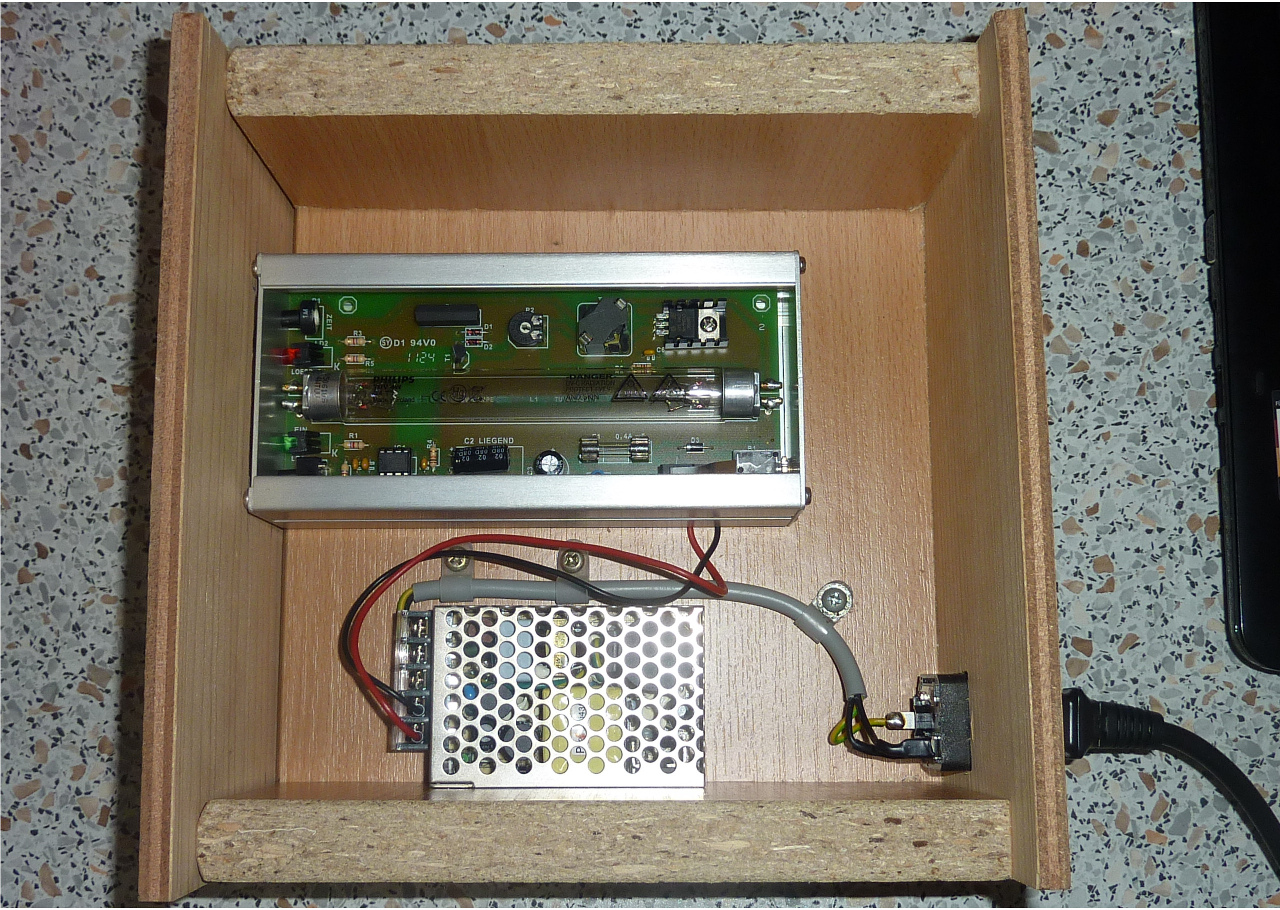
\includegraphics[width=0.67\textwidth]{Bilder/UV-Loeschgeraet.jpg}
\caption{UV-L�schger�t f�r EPROMs (eingebaut in eine Holzkiste)}
\label{fig:UVLoeschgeraet}
\end{figure}

\begin{figure}[h]
\centering
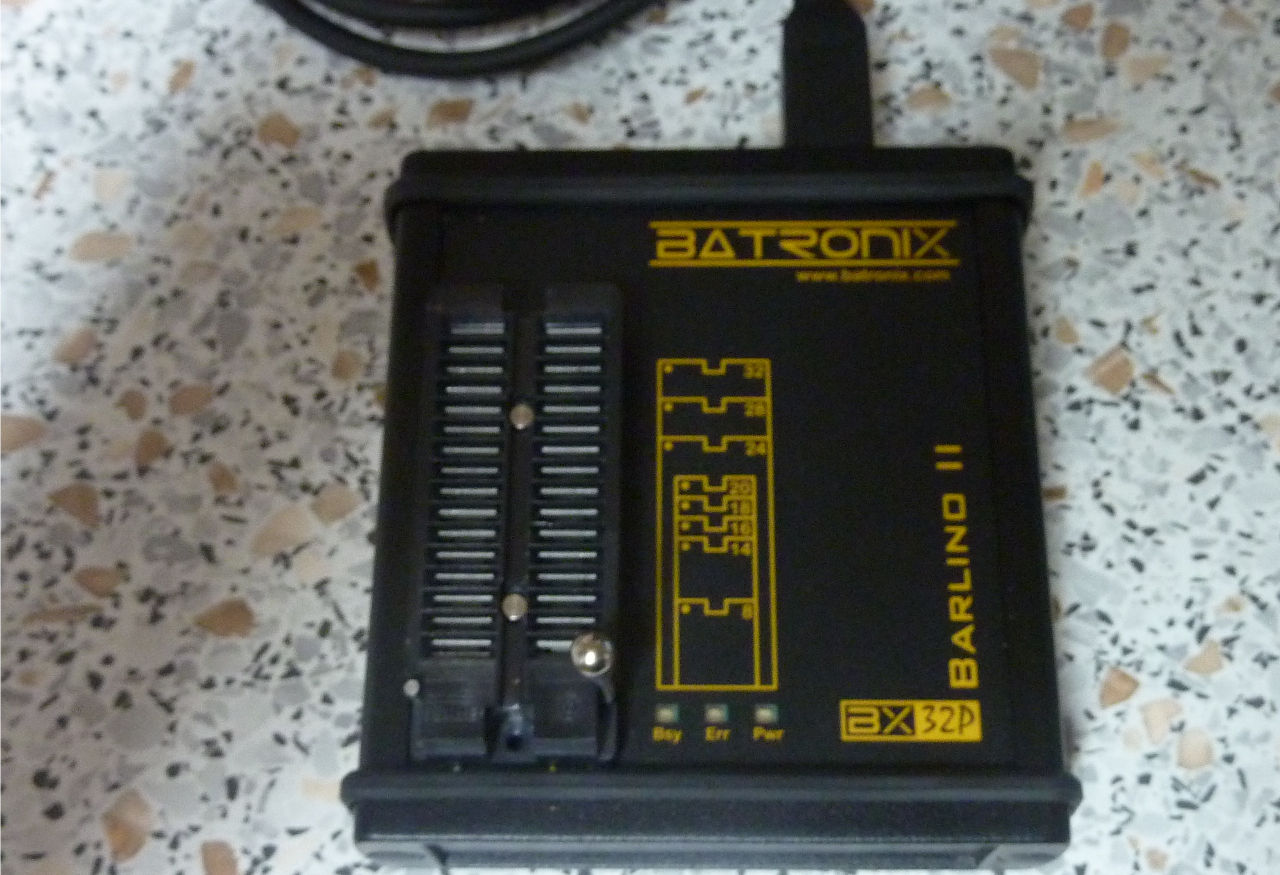
\includegraphics[width=0.67\textwidth]{Bilder/Programmiergeraet.jpg}
\caption{EPROM-Programmierger�t}
\label{fig:Programmiergeraet}
\end{figure}

\begin{figure}[!h]
\centering
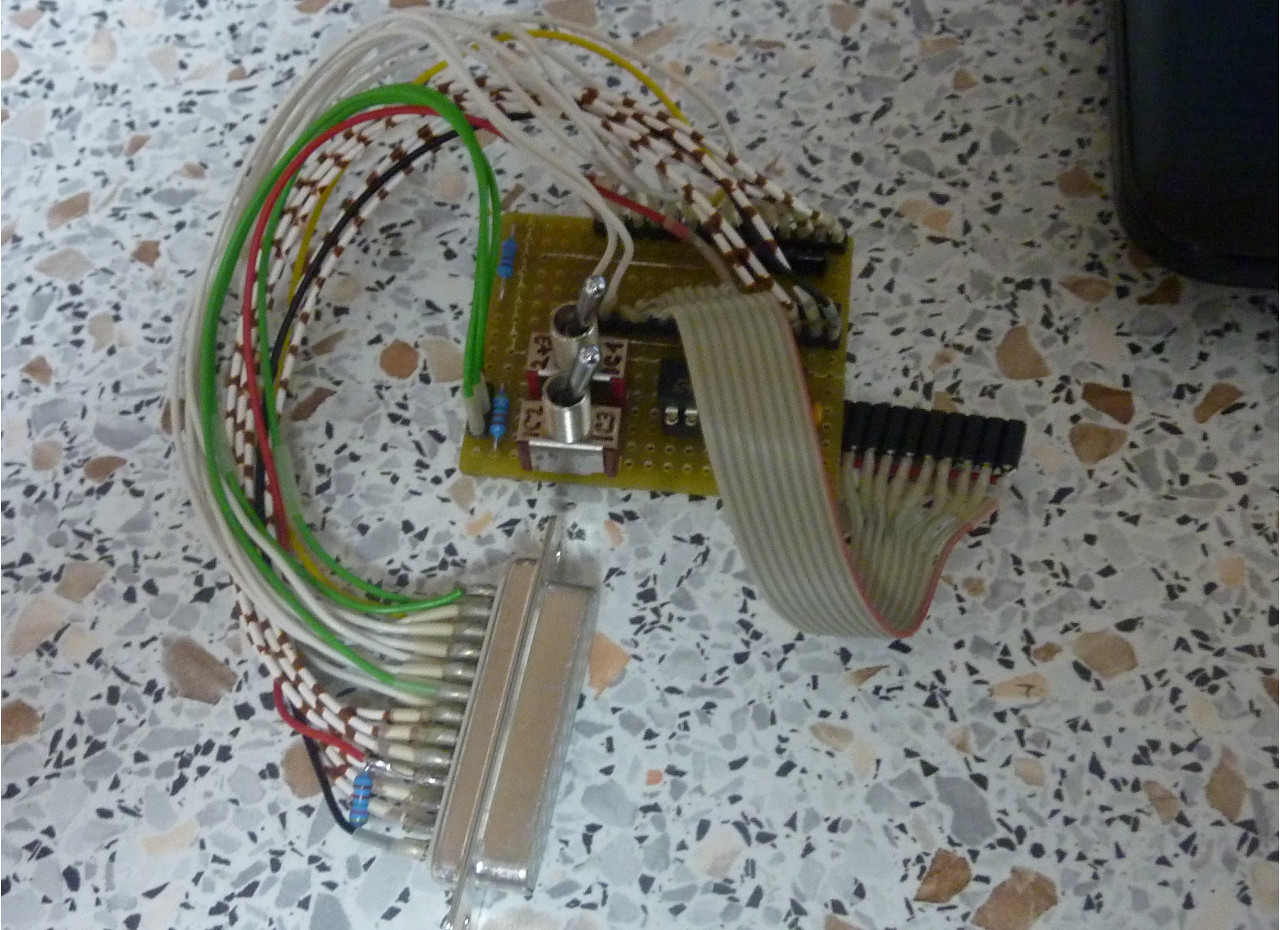
\includegraphics[width=0.67\textwidth]{Bilder/Adapter.jpg}
\caption{Adapter zur Programmierung der EPROMs auf den Modulen}
\label{fig:Adapter}
\end{figure}

\section{Vorbereitung und Umbau der Module f�r Zugriff �ber \Batronix}
{\LARGE Abschnitt entfernt}
%Da auf den EPROM-Modulen bis zu drei EPROMs fest verl�tet sind, aber auf
%dem verwendeten Programmierger�t {\Batronix} die Bausteine normalerweise
%direkt auf den Nullkraftsockel gesteckt werden m�ssen, musste eine
%Adaptierung gebaut werden, an die das EPROM-Modul angesteckt werden
%kann. Die zu programmierenden EPROMs (IC1, IC2 und IC3) auf dem Modul
%k�nnen somit �ber den 25-poligen SUB-D-Stecker des Moduls und �ber eine
%im Modul nachger�stete 10-polige Stiftleiste kontaktiert werden.\\
%Mittels Kippschaltern auf der Adaptierung wird der zu programmierende
%EPROM (IC1, IC2 oder IC3) ausgew�hlt. Dabei wird das Signal CE (Pin 20)
%so beschaltet, wie es auch im Realbetrieb �ber den {\FLTester} erfolgt.\\
%Ferner m�ssen die Ausg�nge des Latchbausteins IC4 (74HC573) w�hrend der
%Programmierung in den hochohmigen Tristate-Modus geschaltet werden,
%damit dessen am Daten- und Adressbus angeschlossenen Ausg�nge nicht
%st�ren. Dies wird durch einen leichten Umbau der Module erreicht:
%Eine als Leiterbahn ausgef�hrte feste Masseverbindung des Enable-Signals
%von IC4 (Pin 1) wird aufgetrennt und durch einen PullDown-Widerstand
%(4k7) ersetzt. Das Enable-Signal ist im Normalbetrieb �ber den PullDown
%weiterhin mit Masse verbunden und damit aktiviert. W�hrend der
%Programmierung kann Enable auf +5V geschaltet werden, um die Ausg�nge
%von IC4 in den gew�nschten Tristate-Modus zu bringen.\\
%Die restlichen Signale des EPROMs sind als 1:1-Verbindungen ausgef�hrt.

\subsection{Programmieradapter f�r die EPROM-Module}
Der Aufbau einer passenden Adaptierung f�r den Programmiervorgang kann
auf einer Lochrasterplatine mit 19 x 15 L�chern aufgebaut werden. Dabei
ist nur darauf zu achten, dass sich der Einbauplatz X100 rechts oben
befindet, damit der Adapter problemlos in den Nullkraftsockel des
Programmierger�tes {\Batronix} gesteckt werden kann, wie es in Abbildung
\ref{fig:AdapterInProgger} dargestellt ist.

\begin{figure}[h]
\centering
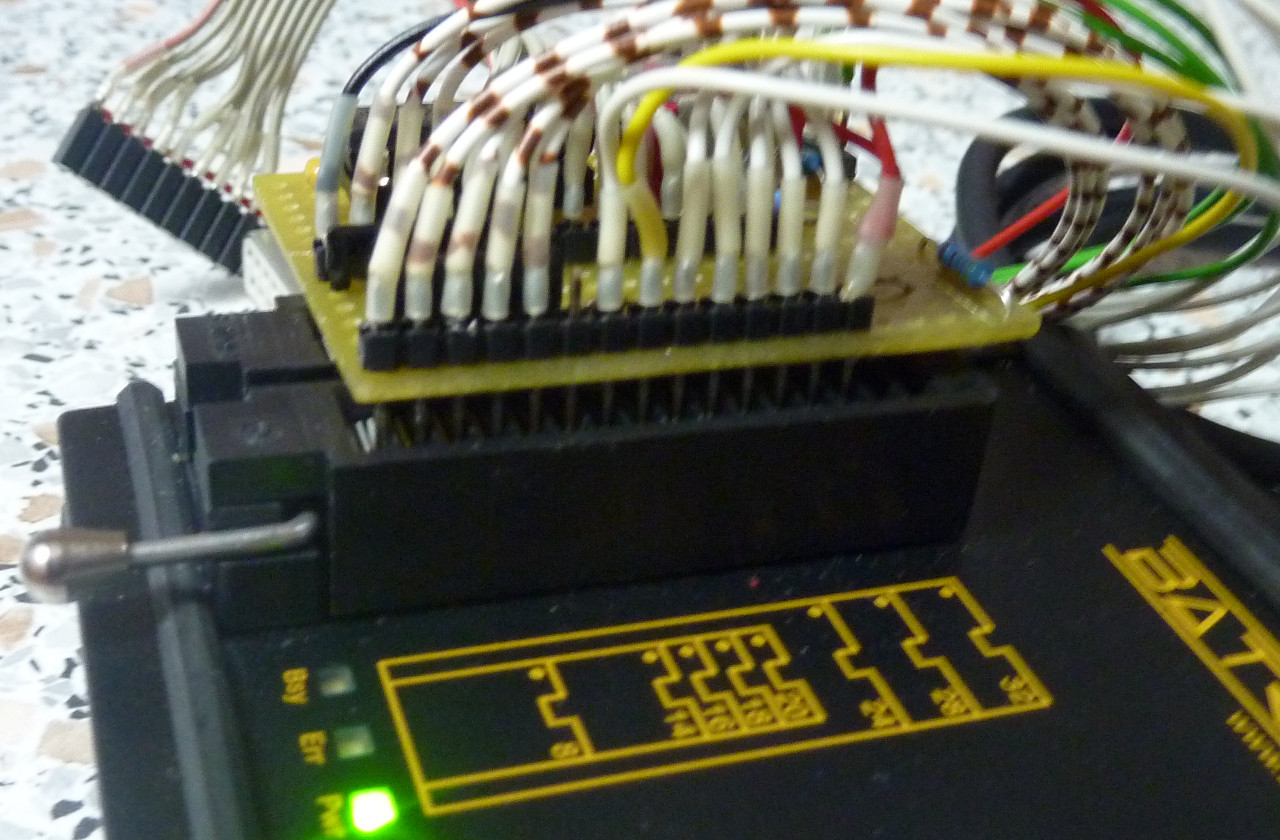
\includegraphics[width=0.67\textwidth]{Bilder/Adapter_auf_Programmiergeraet.jpg}
\caption{Adapter auf Programmierger�t {\Batronix}}
\label{fig:AdapterInProgger}
\end{figure}

Die Kontaktierung erfolgt...
% einerseits �ber eine 25-polige SUB-D-Buchse
%(X1), die an den SUB-D-Stecker des EPROM-Moduls angesteckt wird.
%Weiterhin ist eine Flachbandleitung (X2) f�r die Adressleitungen A0-A7
%auf eine 10-polige Stiftleiste im Inneren des Moduls zu stecken. Daf�r
%muss das EPROM-Modul wie im Abschnitt \ref{subsect:Umbau} beschrieben
%umgebaut werden.

{\LARGE Abschnitt entfernt}


Die Programmierung der bis zu drei in den Modulen verbauten EPROMs
erfolgt f�r jeden Baustein einzeln und getrennt. Sowohl in der
Programmiersoftware {\ProgExpress} als auch auf dem Adapter muss der zu
programmierende Baustein (IC1, IC2 oder IC3) richtig ausgew�hlt werden.
Auf dem Programmieradapter erfolgt die Auswahl �ber die richtige
Schalterstellung der beiden Kippschalter S101 und S102:

\begin{figure}[h]
\centering
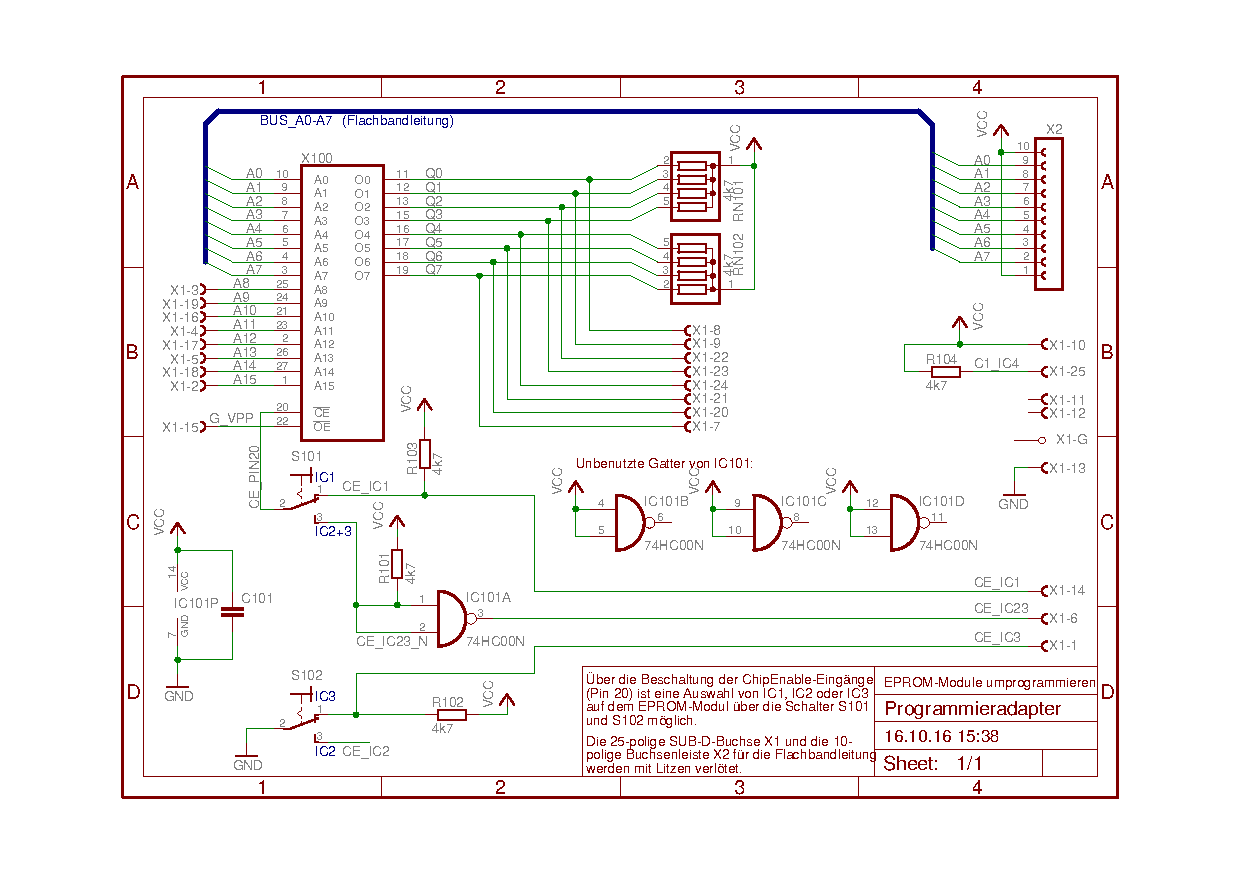
\includegraphics[width=\textwidth]{Bilder/Programmieradapter_sch.pdf}
\caption{Schaltplan des Programmieradapters}
\label{fig:Programmieradapter_sch}
\end{figure}

\begin{figure}[!h]
\centering
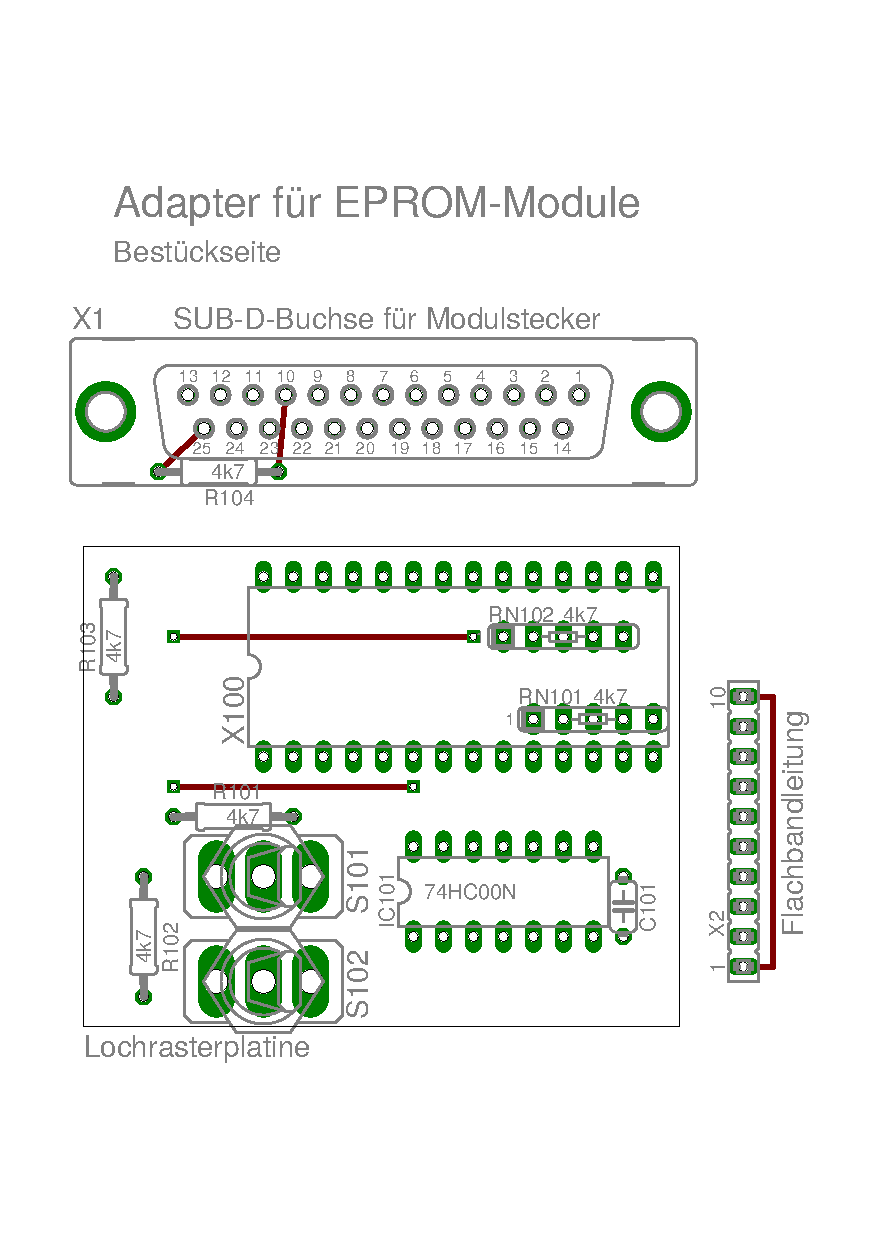
\includegraphics[width=0.49\textwidth]{Bilder/Programmieradapter_top.pdf}
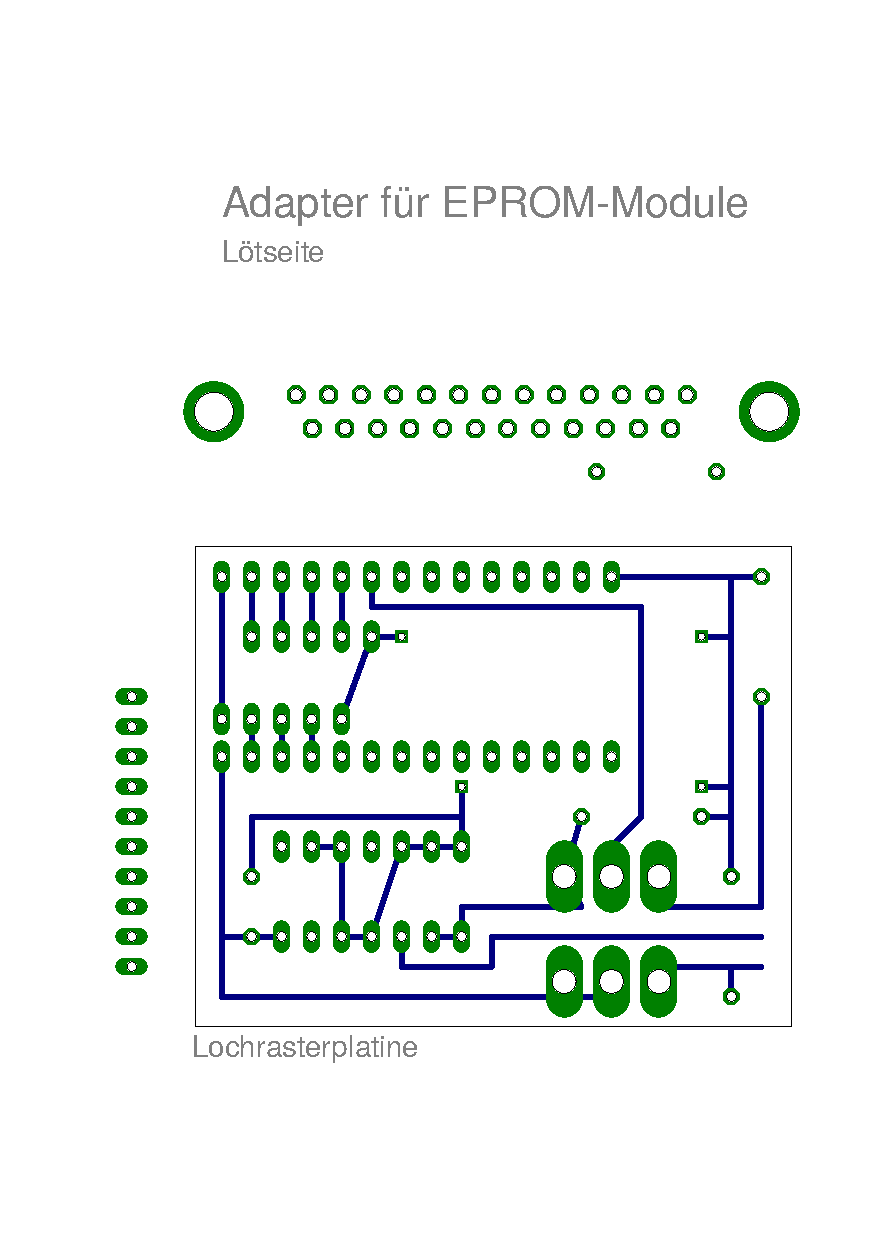
\includegraphics[width=0.49\textwidth]{Bilder/Programmieradapter_bot.pdf}
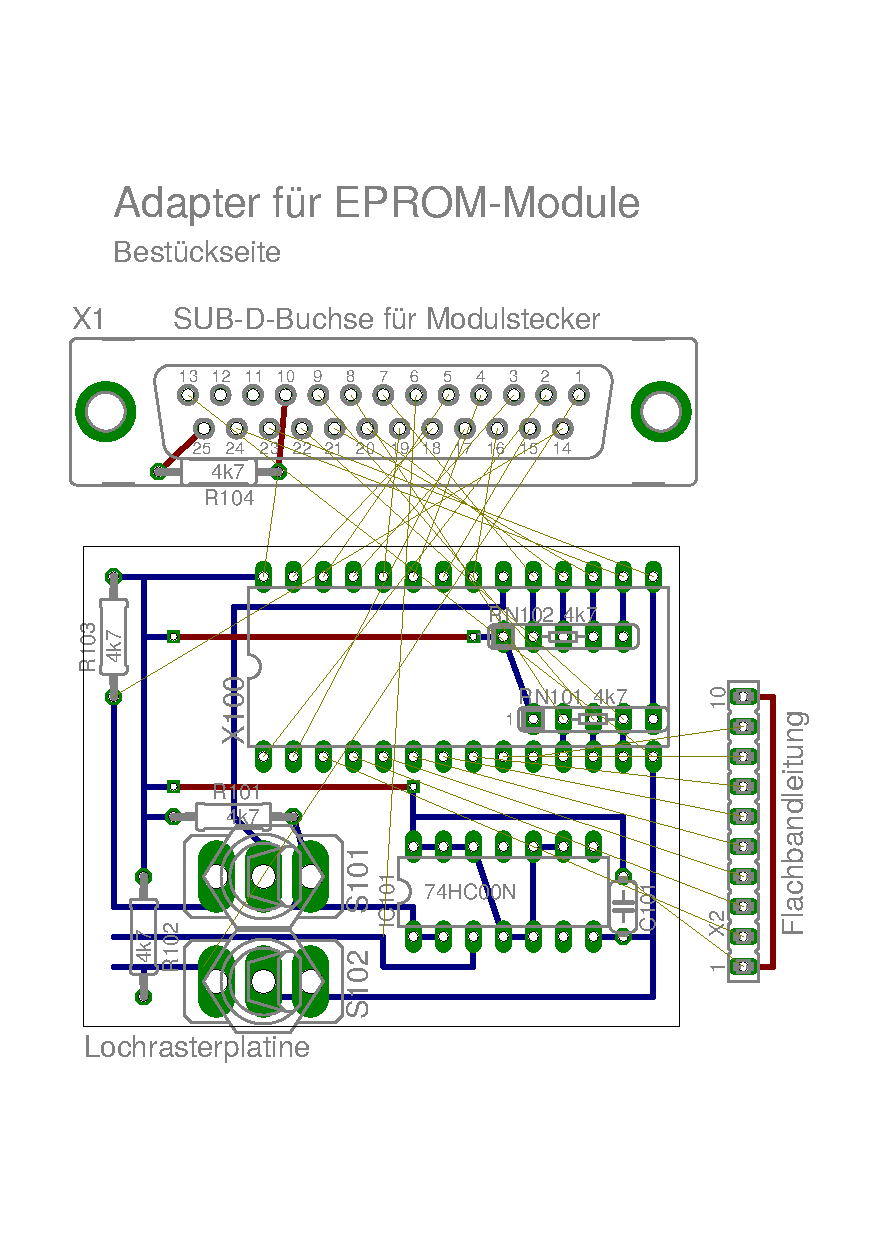
\includegraphics[width=0.49\textwidth]{Bilder/Programmieradapter_brd.pdf}
\caption{Layout des Programmieradapters}
\label{fig:Programmieradapter_layout}
\end{figure}

S101 erm�glicht die Auswahl "`IC1"' oder "`IC2+3"'. In der Stellung 
"`IC1"' wird immer IC1 des Moduls angesprochen. Es ist egal in welcher
Stellung S102 steht.\\
S102 dient der Auswahl "`IC2"' oder "`IC3"'. Dabei darf S101
\textit{nicht} in Stellung "`IC1"' stehen!\\
Siehe Abbildung \ref{fig:Adapter}

In den Abbildungen \ref{fig:Programmieradapter_sch} und 
\ref{fig:Programmieradapter_layout} werden der Schaltplan und eine
m�gliche Umsetzung auf einer Lochrasterplatine illustriert. Abbildung
\ref{fig:Programmieradapter_Fotos} zeigt weitere Fotos von der fertigen
Lochrasterplatine des Programmieradapters.

\begin{figure}[!h]
\centering
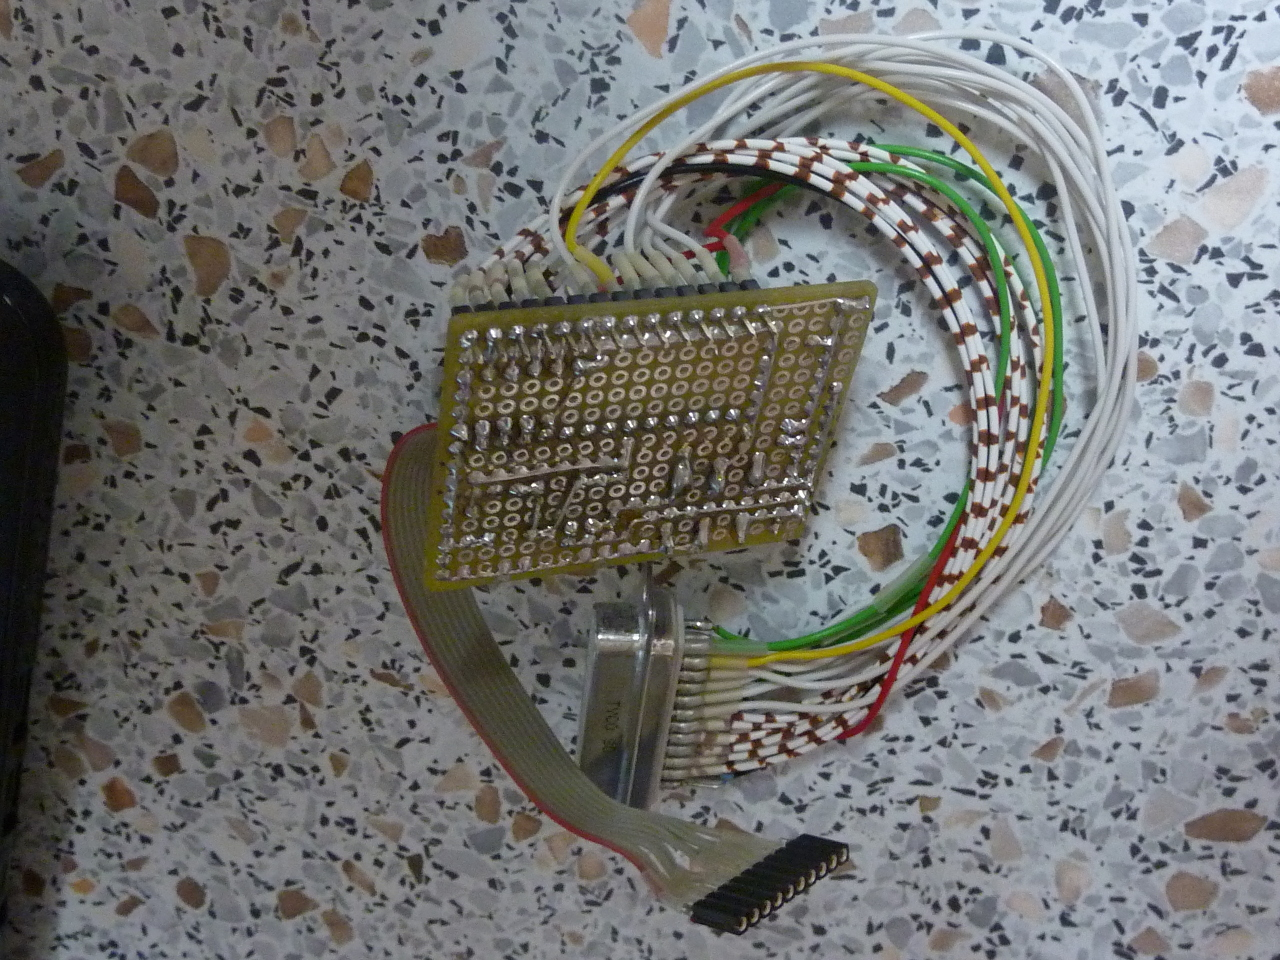
\includegraphics[width=0.49\textwidth]{Bilder/Adapter01.jpg}
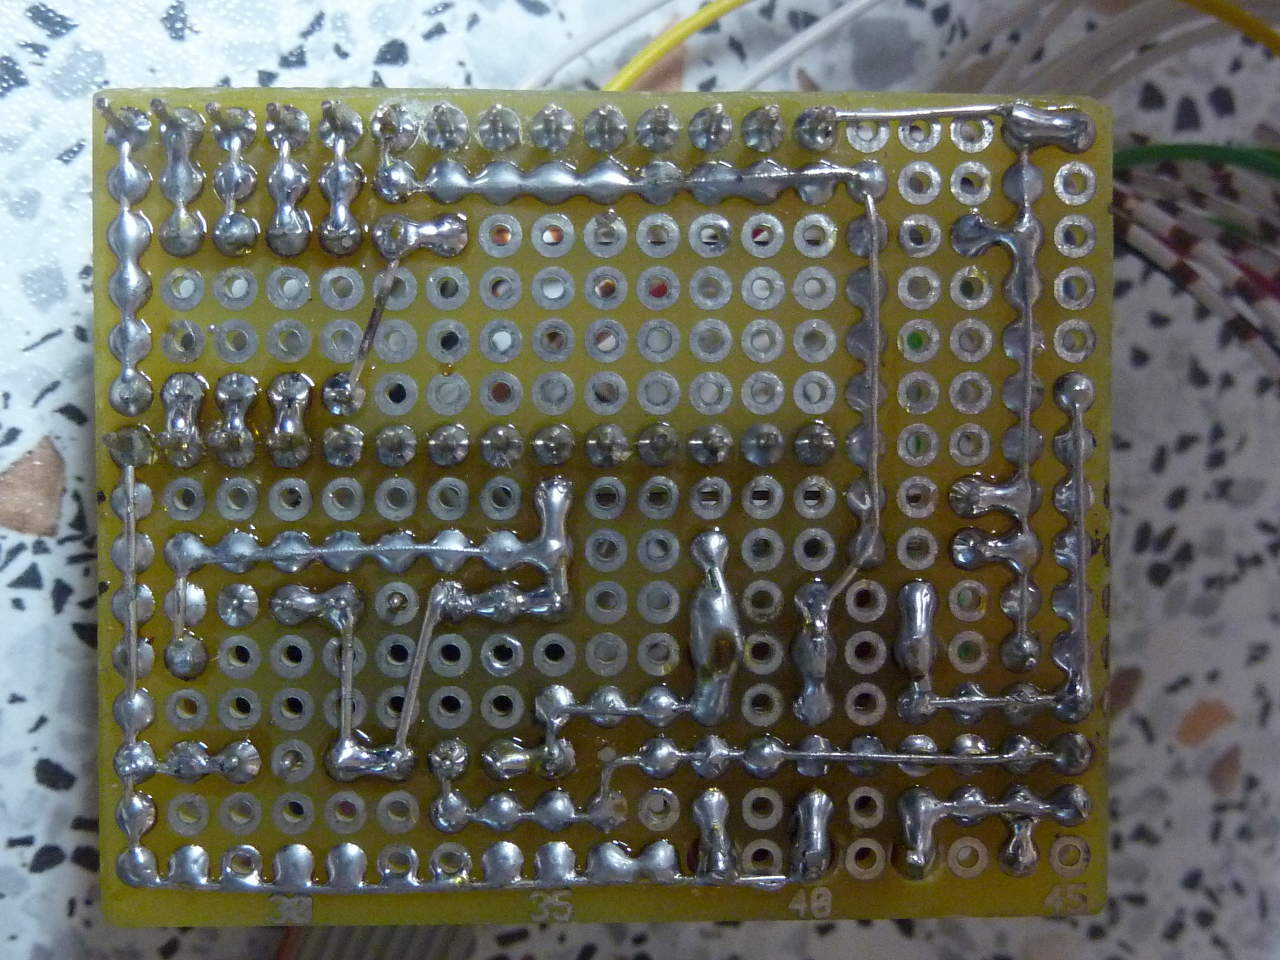
\includegraphics[width=0.49\textwidth]{Bilder/Adapter02.jpg}
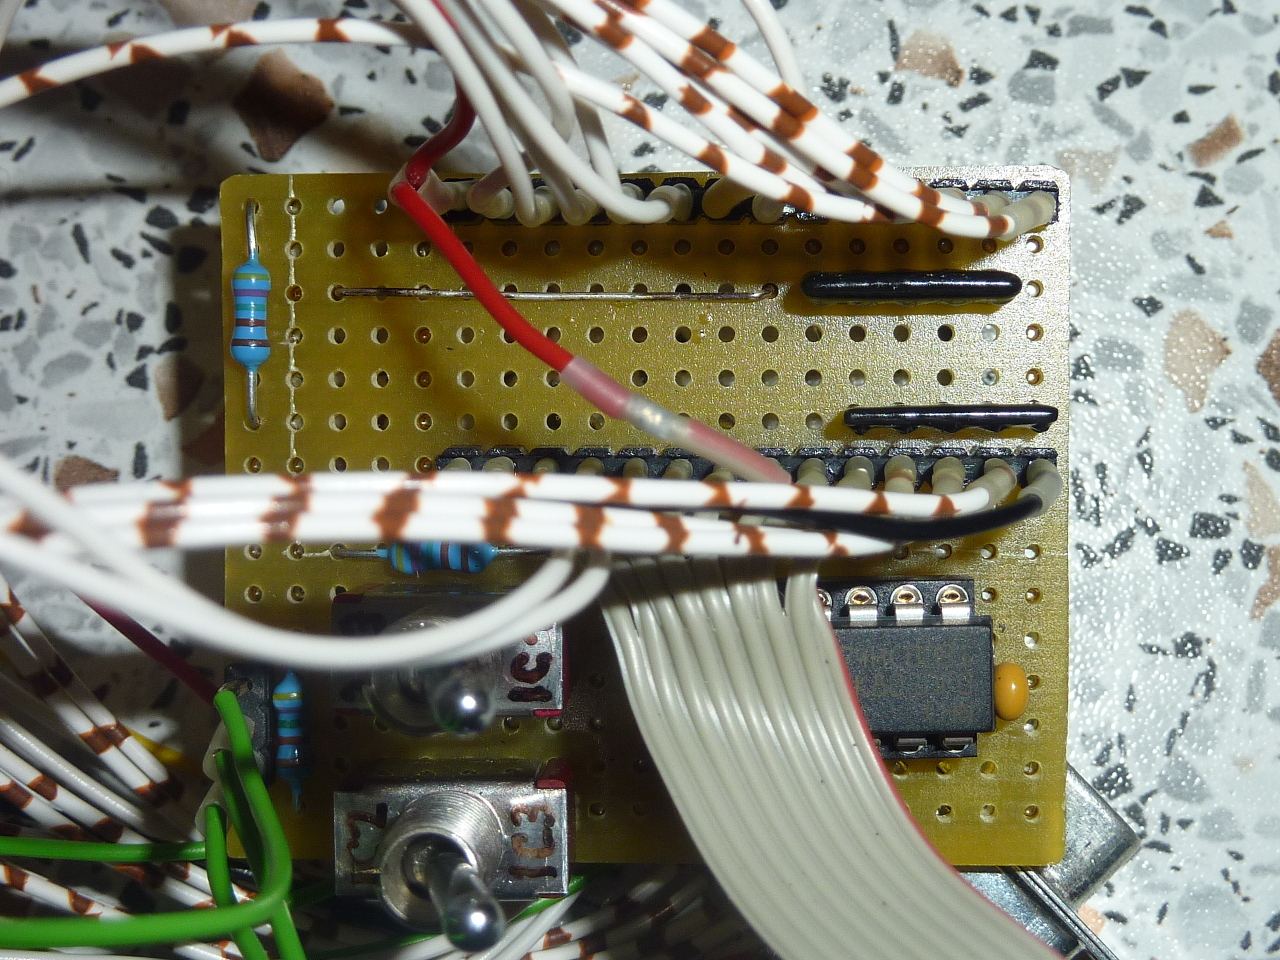
\includegraphics[width=0.49\textwidth]{Bilder/Adapter03.jpg}
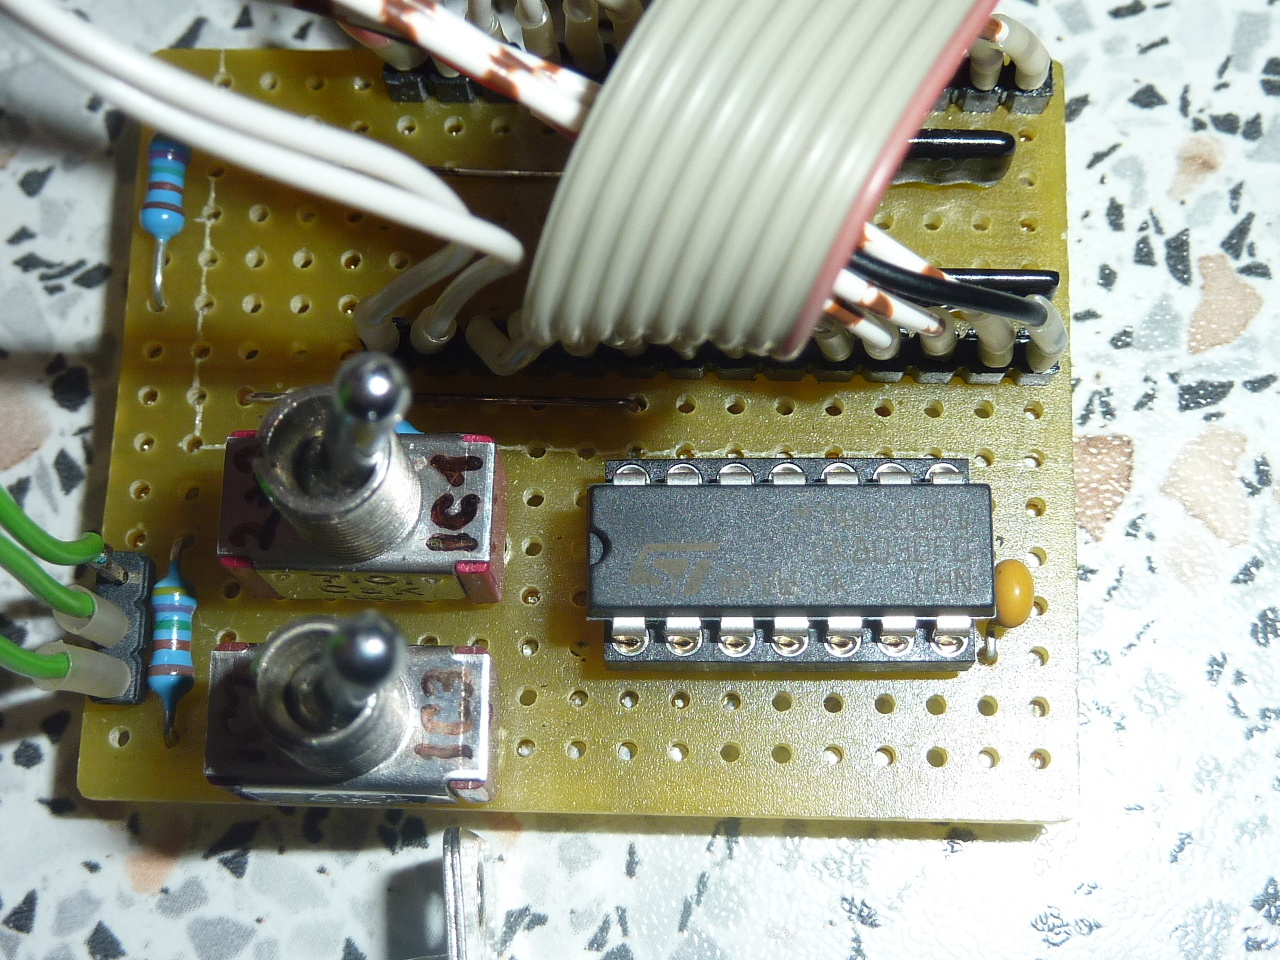
\includegraphics[width=0.49\textwidth]{Bilder/Adapter04.jpg}
\caption{Fotos des Programmieradapters}
\label{fig:Programmieradapter_Fotos}
\end{figure}


\newpage
\subsection{Umbau der Leiterplatten der EPROM-Module}
\label{subsect:Umbau}
Damit die EPROM-Module �ber das hier beschriebene Verfahren neu
programmiert werden k�nnen, sind folgende Umbauma�nahmen an den Modulen
vorzunehmen:

\begin{tabular}{ll}
1. & ... (entfernt)\\
2. & ... (entfernt)\\
3. & ... (entfernt)\\
%1. & Einl�ten der 10-poligen Stiftleiste an einem vorhandenem Einbauplatz\\
%2. & Auftrennen der Leiterbahn f�r die Masseverbindung zu IC4 Pin 1\\
%3. & PullDown-Widerstand (4k7) zu IC4 Pin 1 f�r Normalbetrieb\\
%   & und Vcc-Verbindung f�r Programmierung herstellen\\
\end{tabular}

Die Umbauma�nahmen sind in Abbildung \ref{fig:Umbau} dargestellt.


\section{Softwareinstallation Batronix Prog-Express (Windows)}
Die Software {\ProgExpress} f�r das Programmierger�t {\Batronix} erfolgt
unter Windows �ber die beiliegende CD, auf welcher die Version 1.6
(Stand 2012) der Software enthalten ist. Der Installationsassistent f�r
Windows ist einfach und selbsterkl�rend. F�r die ebenfalls auf der CD
vorhandene Linux-Variante muss zus�tzlich die %quelloffene 
Linux-Implementierung des .NET-Frameworks, \textit{Mono} installiert
werden (\url{http://www.mono-project.com}).

\begin{figure}[!b]
\centering
\includegraphics[width=0.9\textwidth]{Bilder/Umbau01.jpg}
\includegraphics[width=0.9\textwidth]{Bilder/Umbau02.jpg}
\caption{umgebaute Leiterplatte eines EPROM-Moduls}
\label{fig:Umbau}
\end{figure}


\section{Auslesen der Module zur Datensicherung}
\label{sect:Auslesen}
Wenn ein Koffer mit EPROM-Modulen f�r den {\FLTester} gekauft wurde, ist
es zun�chst erforderlich, die Daten auf den Modulen auszulesen und auf
dem  PC zu sichern. 
\begin{bclogo}[logo = \bclampe, noborder = true]{Hinweis}
Die EPROM-Module m�ssen \textit{vor} dem Auslesen der Moduldaten so
umgebaut werden, wie in Kapitel \ref{subsect:Umbau} beschrieben!
\end{bclogo}
Der Anschluss des umgebauten Moduls muss wie in Abbildung
\ref{fig:Modulanschluss} dargestellt erfolgen:

{\LARGE Teilabschnitt entfernt}

%\begin{itemize}
%\item{Das Programmierger�t {\Batronix} an einen USB-Port des PCs anschlie�en.}
%\item{Die Programmieradaptierung in den Nullkraftsockel des Programmierger�tes stecken. Dabei auf die Ausrichtung aus Abbildung \ref{fig:AdapterInProgger} achten.
%\item{Die SUB-D-Stecker sind anzustecken}
%\item{Die Flachbandleitung muss auf die eingel�tete Stiftleiste des Moduls gesteckt werden. F�r die richtige Pinzuordnung muss das Flachbandkabel \textit{ohne Drehung} gesteckt werden!}
%\end{itemize}

\begin{figure}[h]
\centering
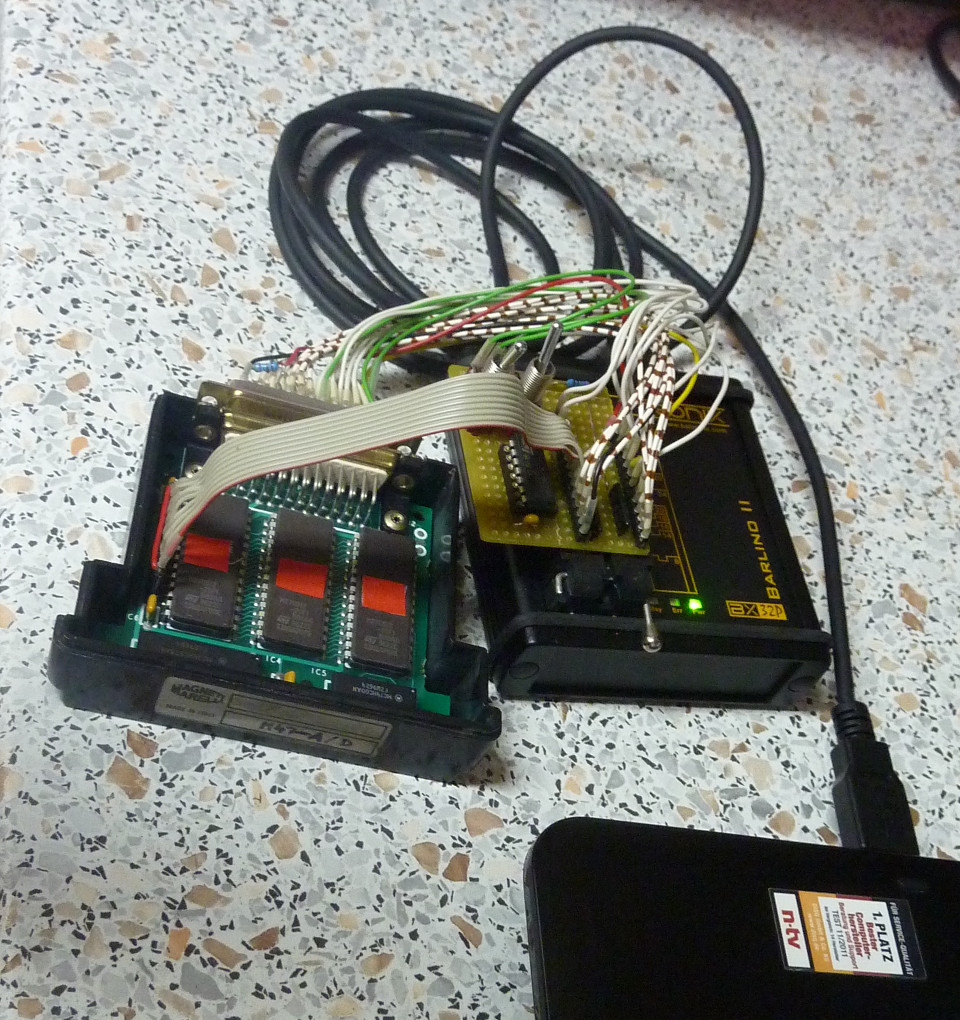
\includegraphics[width=0.67\textwidth]{Bilder/Modulanschluss.jpg}
\caption{Anschluss eines EPROM-Moduls �ber den Programmieradapter am Programmierger�t {\Batronix}}
\label{fig:Modulanschluss}
\end{figure}

Beim Auslesen der Moduldaten sind...

{\LARGE Abschnitt entfernt}
% drei Lesel�ufe f�r IC1, IC2 und IC3
%erforderlich. Auf IC1 k�nnen nur 8KByte gespeichert (und ausgelesen)
%werden, daher muss in den Chip-Optionen f�r IC1 der auszulesende
%Speicherbereich von Startadresse 0 bis Endadresse 0x1FFF (8191 dez.)
%gesetzt werden!\\
%IC2 und IC3 enthalten Daten im gesamten Speicherbereich (64KByte) des
%Bausteins (27C512). Es gibt auch Leiterplatten mit kleineren EPROMs
%(\zB 27C256 mit 32KByte). In diesem Falle kann der Bausteintyp entweder
%�ber die Funktion "`Chip Autoerkennung"' der Programmiersoftware
%ermittelt werden, dann wird seine Speichergr��e von der Software
%automatisch korrigiert oder der Speicherbereich wird auch hier manuell
%eingeschr�nkt.\\
%Die ausgelesenen Daten werden zweckm��igerweise in einem Ordner mit dem
%Modulnamen (\zB "`M23A"') unter den Dateinamen \texttt{IC1.bin},
%\texttt{IC2.bin} und \texttt{IC3.bin} abgelegt.

\subsection*{Auslesevorgang �ber die Software {\ProgExpress}}
Die Oberfl�che der Software {\ProgExpress} ist im Wesentlichen in drei
Spalten konzipiert. Links befinden sich die m�glichen Aktionen als
Piktogramme. In der Mitte (Hauptteil) wird die gew�hlte Aktion im Detail
angezeigt: Oben die genaue Parametrierung und im unteren Teil die
Einzelschritte der Aktion. Durch Anklicken der einzelnen Elemente k�nnen
notwendige  Anpassungen vorgenommen werden. Der rechte Teil enth�lt ein
Log-Fenster, in dem alle durchgef�hrten Aktionen mit Ergebnis angezeigt
werden.

\begin{figure}[h]
\centering
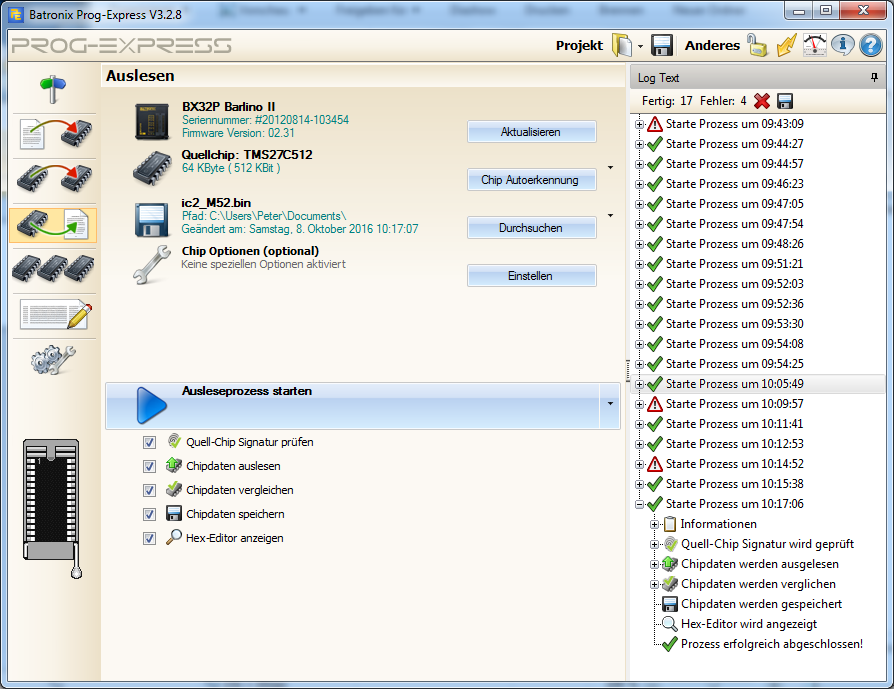
\includegraphics[width=0.9\textwidth]{Bilder/Prog-Express_Auslesen_IC2.png}
\caption{Grundlegende Softwareeinstellungen zum Auslesen der EPROM-Daten}
\label{fig:SoftEinstellungen}
\end{figure}

Zum Auslesen der Moduldaten sind in  folgende Schritte
notwendig:
Zun�chst muss in der Software im linken Bereich die richtige Aktion, 
hier das Auslesen der Chipdaten durch Anklicken des entsprechenden
Piktogramms gew�hlt werden.\\

\includegraphics[]{Bilder/Prog-Express_Auslesen_icon.png}

{\LARGE Abschnitt entfernt}
%In bestimmten F�llen, insbesondere bei IC1, von dem aufgrund seiner
%Beschaltung in den EPROM-Modulen nur ein Block von 8KByte adressiert
%werden kann, muss in den Chip-Optionen die Speichergr��e angepasst
%werden, siehe Abbildungen \ref{fig:SoftEinstellungenIC1} und
%\ref{fig:SoftEinstellungenIC1addr}\\
%Bei IC2 und IC3 m�ssen dagegen die kompletten Speicherbereiche
%ausgelesen werden! Dazu vor dem Ausleseprozess in den Chip-Optionen die
%Einschr�nkung des Adressbereichs von IC1 wieder deaktivieren. Die
%Software {\ProgExpress} verwendet bei der richtigen Auswahl des Chiptyps
%die richtige Speichergr��e.

\begin{figure}[h]
\centering
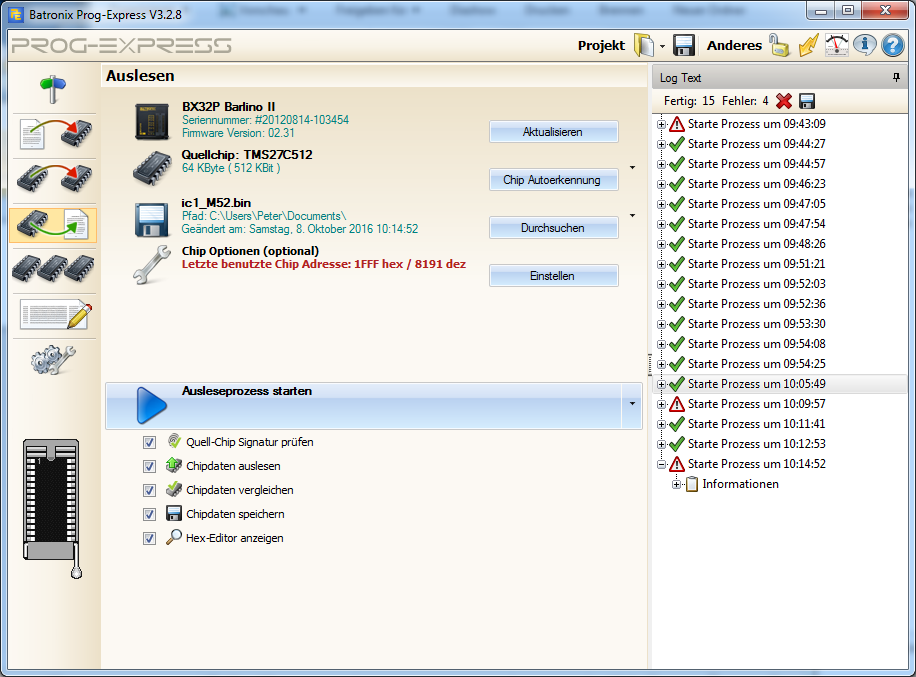
\includegraphics[width=0.92\textwidth]{Bilder/Prog-Express_Auslesen_IC1_8kB.png}
\caption{Softwareeinstellungen zum Auslesen von IC1 (max. 8KByte)}
\label{fig:SoftEinstellungenIC1}
\end{figure}

Auf den einzelnen Modulen k�nnen folgende EPROM-Typen verbaut sein:\\
\begin{tabular}{ll}
M27C64  & 8KByte Speicherkapazit�t\\
M27C256 & 32KByte Speicherkapazit�t\\
M27C512 & 64KByte Speicherkapazit�t\\
\end{tabular}
\\ \\ Der Auslesevorgang dauert pro Baustein nur ca. 1 Sekunde.
\begin{bclogo}[logo = \bclampe, noborder = true]{Hinweise}
Um die \textit{vollst�ndigen} Daten eines EPROM-Moduls zu erhalten,
m�ssen logischerweise \textit{alle} best�ckten EPROMs (IC1, IC2 und IC3)
ausgelesen werden!\\
F�r IC2 und IC3 muss unbedingt darauf geachtet werden, deren
\textit{gesamten} Speicherbereich auszulesen!\\
Die Schalter S101 und S102 auf dem Programmieradapter sind \textit{vor}
dem Auslesevorgang in die richtige Schaltstellung zu bringen!
\end{bclogo}

\begin{figure}[h]
\centering
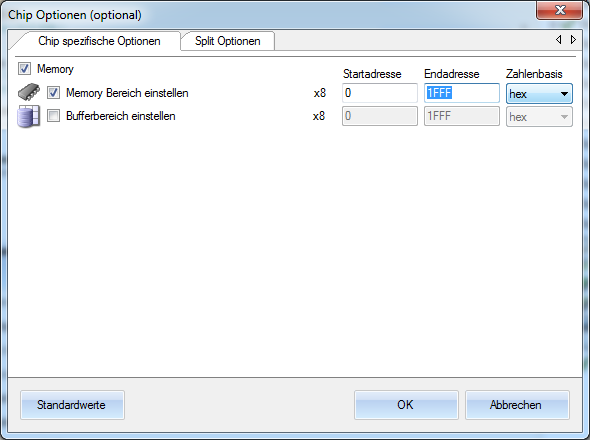
\includegraphics[width=0.6\textwidth]{Bilder/Prog-Express_IC1_8kB.png}
\caption{Parametrierung des gew�nschten Adressbereichs von IC1 (8KByte)}
\label{fig:SoftEinstellungenIC1addr}
\end{figure}


\section{L�schen der Module mit UV-Licht}
\label{sect:Loeschen}
In den EPROM-Modulen wurden die klassischen EPROMS verbaut, die nur mit
UV-Licht gel�scht werden k�nnen. Dazu wird ein EPROM-L�schger�t mit
UV-Lampe (Abbildung \ref{fig:UVLoeschgeraet}) verwendet, das aus
Sicherheitsgr�nden in eine lichtundurchl�ssige Holzkiste eingebaut
wurde.
\begin{bclogo}[arrondi = 0.2, logo = \bcinfo, ombre = true, epOmbre = 0.25, couleurOmbre = black !30,blur]{Achtung}
Das vom EPROM-L�schger�t abgegebene UV-Licht kann die Haut und vor allem
die Augen schwer sch�digen! Daher darf das L�schger�t \textbf{nur im
geschlossenen Zustand} betrieben werden!
\end{bclogo}
Vor dem Programmieren eines EPROM-Moduls mit neuen Daten m�ssen zun�chst
die vorhandenen Daten von den EPROMs gel�scht werden. Dazu muss der
Deckel der Holzkiste abgenommen werden und eine oder zwei Leiterplatten
von ge�ffneten EPROM-Modulen �ber die UV-Lampe des L�schger�tes gelegt
werden. Dabei darf nicht vergessen werden, die Lichtschutzaufkleber von
den runden Quarzglasfenstern der EPROMs zu entfernen!\\
Vor dem Einschalten des L�schger�tes muss aus Gr�nden des Eigenschutzes
unbedingt der Holzdeckel geschlossen werden.\\
Der L�schvorgang unter UV-Licht dauert ca. 20 -- 30 Minuten. Bei
k�rzeren Belichtungszeiten k�nnen einzelne Bits stehen bleiben, die dann
bei der nachfolgenden Neuprogrammierung st�ren! Nach dem L�schvorgang
sollte vor der Neuprogrammierung nochmals f�r mindestens die gleiche
Zeit gewartet werden, um die soeben gel�schten EPROMs "`abk�hlen"' zu
lassen.
\begin{bclogo}[logo = \bclampe, noborder = true]{Hinweis}
Technisch gesehen erfolgt das L�schen �ber eine Ionisation des
Halbleitermaterials durch das UV-Licht, die die gespeicherten
Ladungstr�ger abflie�en l�sst. Diese Ionisation kann nach dem Abschalten
des UV-Lichtes noch einige Zeit anhalten, wenn auch in geringerem Ma�e,
aber m�glicherweise daf�r ausreichend, dass die durch eine unmittelbar
folgende Programmierung neu aufgebrachten Ladungstr�ger zumindest
teilweise wieder abflie�en. Dies kann sich nach au�en dann durch 
kippende Bits oder eine verk�rzte Datenlebensdauer bemerkbar machen.
\end{bclogo}
Ein vollst�ndig gel�schtes EPROM enth�lt nur Bits mit dem bin�ren Wert
"`1"'. Beim Programmiervorgang werden ausschlie�lich "`0"'-Bits
programmiert, die "`1"'-Bits bleiben leer ("`unprogrammiert"'). Details
zur Technologie von EPROMs befinden sich hier:\\
\url{https://de.wikipedia.org/wiki/Erasable_Programmable_Read-Only_Memory}


\section{Programmieren der Module mit (neuen) Daten}
{\LARGE Abschnitt entfernt}

%Auch beim Programmieren von EPROM-Modulen sind drei Durchl�ufe f�r IC1,
%IC2 und IC3 erforderlich. Aufgrund der internen Beschaltung im Modul
%k�nnen auf IC1 nur 8KByte gespeichert werden, daher muss in den
%Chip-Optionen f�r IC1 der zu programmierende Speicherbereich von
%Startadresse 0 bis Endadresse 0x1FFF (8191 dez.) gesetzt werden!\\
%IC2 und IC3 k�nnen dagegen �ber ihren gesamten Speicherbereich
%adressiert und programmiert werden.\\
Grunds�tzlich gelten die f�r das Auslesen der EPROM-Module relevanten
Punkte (siehe Kapitel \ref{sect:Auslesen}) auch f�r die Programmierung.

\subsection*{Programmiervorgang �ber die Software {\ProgExpress}}
Zum Programmieren der Moduldaten sind in  folgende Schritte
notwendig:
Zun�chst muss in der Software im linken Bereich die richtige Aktion, 
hier das Programmieren der Chipdaten durch Anklicken des entsprechenden
Piktogramms gew�hlt werden.\\

\includegraphics[]{Bilder/Prog-Express_Programmieren_icon.png}

Vor der Programmierung sollte unbedingt kontrolliert werden, ob in der
Software die richtige Programmierdatei gew�hlt wurde und ob die Schalter
S101 und S102 auf dem Programmieradapter in der richtigen Stellung sind.
W�hrend solche Fehler beim Auslesen -- sofern rechtzeitig bemerkt --#
noch relativ unproblematisch sind, sollten sie beim Programmieren auf
jeden Fall vermieden werden, da ein falsch programmierter EPROM erst
wieder \textit{m�hsam} gel�scht werden muss (siehe Kapitel
\ref{sect:Loeschen})!

\begin{figure}[h]
\centering
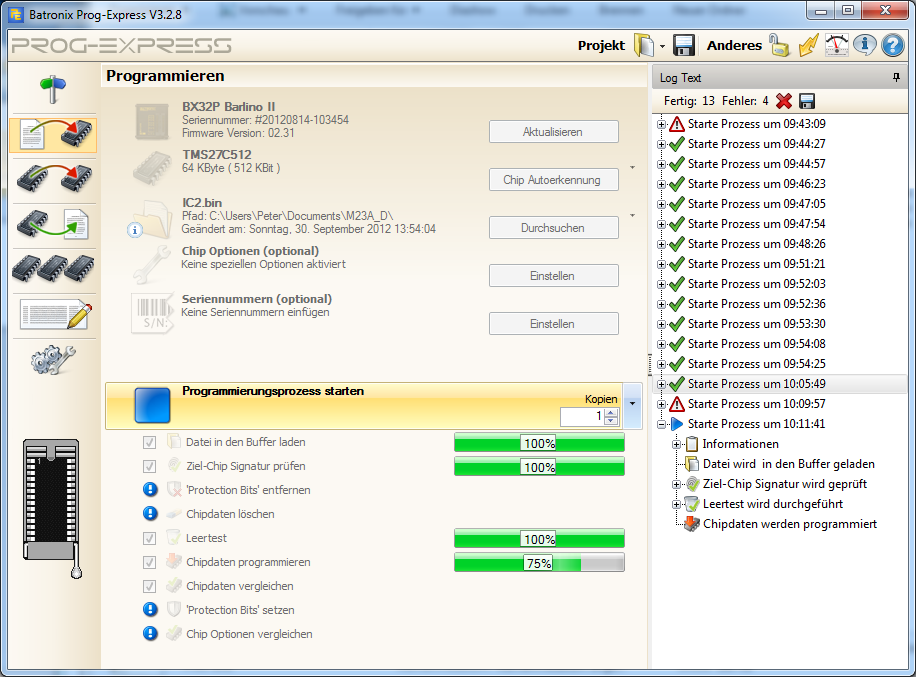
\includegraphics[width=0.92\textwidth]{Bilder/Prog-Express_Einstellungen_IC2.png}
\caption{Softwareeinstellungen zum Programmieren von IC2}
\label{fig:SoftEinstellungenIC2}
\end{figure}

Der Programmiervorgang dauert nur wenige Sekunden, ist aber etwas
langsamer als der Auslesevorgang. Wichtig ist der Schritt "`Leertest"'
vor der Programmierung. Dort wird �berpr�ft, ob wirklich jede
Speicherstelle des EPROMs gel�scht ist, \dahe nur "`1"'-Bits enth�lt.
Wenn dies nicht der Fall ist, muss das Modul zuvor erst gel�scht werden!
Diese Pr�fung und der Vergleich der Chipdaten stellen sicher, dass die
programmierten Daten wirklich korrekt im EPROM abgelegt sind.



% ##############################################################################
% ------------------------------------------------------------------------------
% ##############################################################################


% ANHANG -----------------------------------------------------------------------
%   Die Inhalte des Anhangs werden analog zu den Kapiteln inkludiert.
%   Dies geschieht in der Datei "Anhang.tex".
% ------------------------------------------------------------------------------
\begin{appendix}
    \clearpage
    \pagenumbering{roman}
    \chapter{Anhang}
    \label{sec:Anhang}
    % Rand der Aufz�hlungen in Tabellen anpassen
    \setdefaultleftmargin{1em}{}{}{}{}{}
    \begin{itemize}
%\item	Abk�rzungsverzeichnis
\item	Stromlaufplan Leiterplatte \textbf{79 63 82 40}
\item	Stromlaufplan Leiterplatte \textbf{79 54 33 50}
\end{itemize}

{\LARGE Der Anhang wurde entfernt}

%%---------------------------------------------------------------
%%  Abk�rzungsverzeichnis
%%---------------------------------------------------------------
%\section{Abk�rzungsverzeichnis}
%Folgende Abk�rzungen werden im Dokument verwendet
%
%\begin{table}[!h]
%\centering
%\renewcommand{\arraystretch}{2}
%\begin{tabular}{|l|l|}
%\hline
%Sepp	&	Sepperl\\
%\hline
%Meldung	&	ndfioshoi\\
%\hline
%Meldung	&	ndfioshoi\\
%\hline
%\end{tabular}
%\vspace{0.5cm}
%\caption{Abk�rzungsverzeichnis}
%\end{table}


%---------------------------------------------------------------
%  Stromlaufpl�ne
%---------------------------------------------------------------
\includepdf[pages=-, portrait, scale=1.0, addtotoc={1,section,0,Stromlaufplan Leiterplatte 79 63 82 40,79 63 82 40} ]{Bilder/FLTester-Modul79638240.pdf}
\includepdf[pages=-, portrait, scale=1.0, addtotoc={1,section,0,Stromlaufplan Leiterplatte 79 54 33 50,79 54 33 50} ]{Bilder/FLTester-Modul79543350.pdf}

%---------------------------------------------------------------
%  geflickter Stromlaufplan (Beispiel)
%---------------------------------------------------------------
%\includepdf[pages=-, portrait, scale=1.0, addtotoc={1,section,0,Schaltplan,Schaltplan} ]{Bilder/Anhang/Schaltplan_S1-2.pdf}
%\includepdf[pages=-, portrait, scale=1.0, addtotoc={0,section,0,Schaltplan,Schaltplan} ]{Bilder/Anhang/Schaltplan_S3.pdf}
%\includepdf[pages=-, portrait, scale=1.0, addtotoc={0,section,0,Schaltplan,Schaltplan} ]{Bilder/Anhang/Schaltplan_S4ff.pdf}

\end{appendix}

% Index ------------------------------------------------------------------------
%   Zum Erstellen eines Index, die folgende Zeile auskommentieren.
% ------------------------------------------------------------------------------
%\printindex

\end{document}
